\chapter{Blockchain}
Le criptomonete, a partire dal 2008\footnote{Anno di pubblicazione del whitepaper di Satoshi Nakamoto}, hanno ricevuto molte attenzioni da coloro che sono interessati ad investirci o costruire nuovi servizi per un guadagno personale ma soprattutto è esploso l'interesse verso la vera innovazione tecnologica su cui sono basate: la \textbf{blockchain}.

Una \textit{blockchain} può essere pensata come un database distribuito e replicato in diversi computer connessi ad una rete.\newline
La principale innovazione introdotta da questa tecnologia è nel protocollo del consenso distribuito usato per gestire transazioni anche su reti a bassa latenza o dispositivi a bassa potenza senza la necessità di un sistema centrale per garantire protezione e affidabilità.

Non esiste una definizione globalmente valida di \textit{blockchain} a causa delle differenti implementazioni e varianti ma è possibile delineare alcuni punti chiave.\newline
Una blockchain è una rete \textit{peer-to-peer} completamente \textit{distribuita} che fa ampio uso di crittografia per eseguire applicazioni, salvare dati, trasferire asset digitali in maniera \textit{sicura}; questa tecnologia può essere vista come un registro pubblico e non controllato da nessuna autorità centrale in cui è solo possibile aggiungere dati (\textbf{append-only}).

Questa definizione è interessante in quanto non menziona nessun termine finanziario o particolari casi d'uso e non specifica protocolli o algoritmi di consenso in quanto una blockchain può essere implementata come un sistema general purpose e non come solo meccanismo per i pagamenti elettronici; infatti, la prima blockchain è stata progettata nel 1991 da due crittografi: \textit{Stuart Haber} e \textit{Scott Stornetta} per firmare dei documenti digitali per prevenire modifiche illecite dei dati e autenticazione.\newline

\section{Storia}
La blockchain utilizzata per i Bitcoin è la prima moderna blockchain ad essere utilizzata per pagamenti elettronici sicuri, distribuiti ed anonimi ed è stata presentata da Satoshi Nakamoto nel 2008. L'esigenza di Satoshi era quella di creare un protocollo decentralizzato per coniare una moneta digitale senza il bisogno di una figura centrale di fiducia ed evitare il problema del \textit{double-spending} di possibili attori malevoli.
Molte altre proposte sono state fatte prima dei Bitcoin ma nessuna risolveva a pieno i problemi di decentralizzazione e consenso distribuito.
\begin{figure}
    \centering
    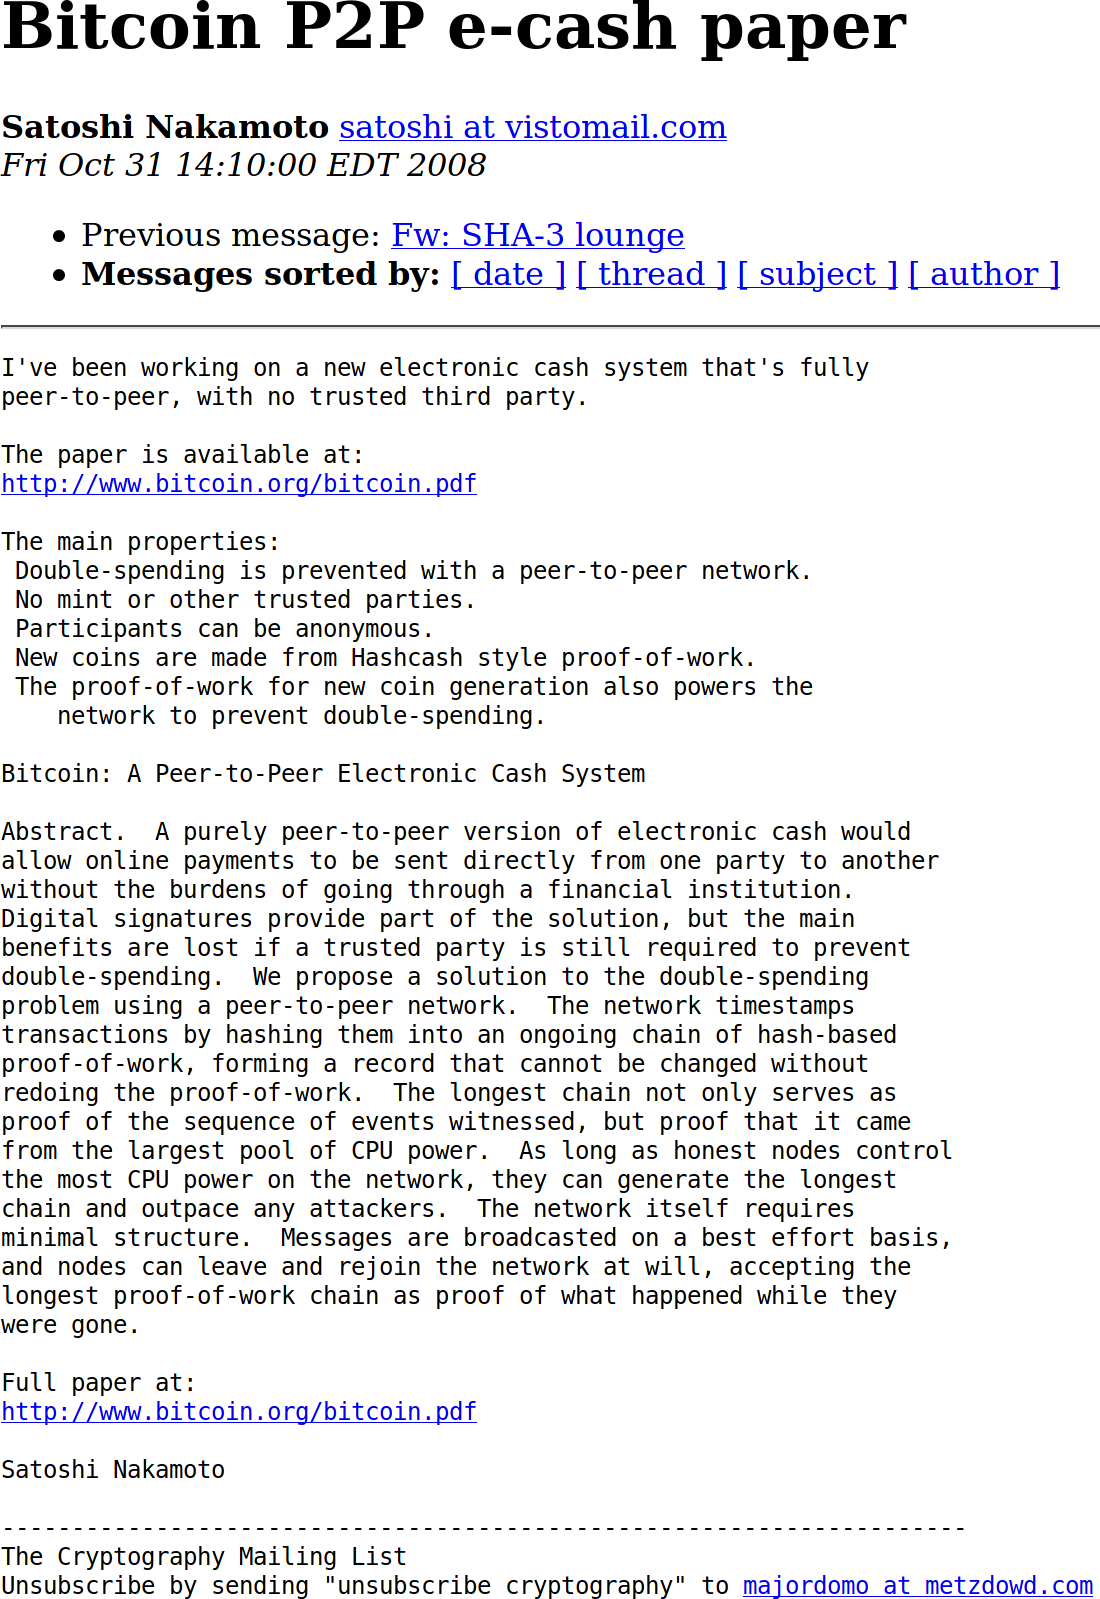
\includegraphics[width=0.6\textwidth]{images/satoshimail.png}
    \caption{La prima mail di presentazione di Bitcoin da parte di Satoshi Nakamoto su una mailing-list di cypherpunk: \href{metzdowd.com}{metzdowd.com}.}
\end{figure}

La prima blockchain conosciuta, però, non è quella implementata per Bitcoin e non è stata usata per pagamenti elettronici ma come metodo di validazione per documenti digitali nel 1991.

\subsection{Haber e Stornetta}
L'idea di Haber e Stornetta\cite{haberstornetta} era di certificare la data di creazione o modifica di un documento; per esempio, in materia di dispute per la proprietà intellettuale è cruciale verificare la data di un prototipo brevettabile: la soluzione richiede di risolvere due problemi.
\begin{itemize}
    \item la data e l'ora devono far parte del timestamp e non solo nel documento;
    \item prevenire ogni modifica del timestamp e quindi del documento.
\end{itemize}
La soluzione proposta dai due crittografi permette di eseguire un timestamp digitale dei documenti in modo tale che sia infattibile per un attaccante alterare questi dati.\newline
Il processo di timestamp di un documento prevede l'utilizzo di funzioni di hashing crittografiche: $h: \{0,1\}^* -> \{0,1\}^l$.\newline
A differenza delle funzioni di hashing presentate nel capitolo \ref{sec:funzioni-hashing} non è necessario che siano resistenti alla seconda preimmagine in quanto la soluzione richiede che da un hash non sia possibile risalire al messaggio originale.
Utilizzando le funzioni di hashing è possibile quindi evitare di fornire l'intero documento ad un servizio per timestamp e quindi garantire la privacy del documento stesso: il contenuto intellettuale non è divulgato pubblicamente.\newline
Una volta che l'hash del documento è stato generato è possibile applicargli una firma digitale.\newline
Una prima soluzione proposta prevede l'utilizzo di un servizio di terze parti (\textit{Time-Stamping Service}) per elaborare e firmare il documento ma sorge il problema della falsificazione: è necessario implementare una soluzione che sia assente da terze parti per garantire il massimo della fiducia.
\begin{figure}
    \centering
    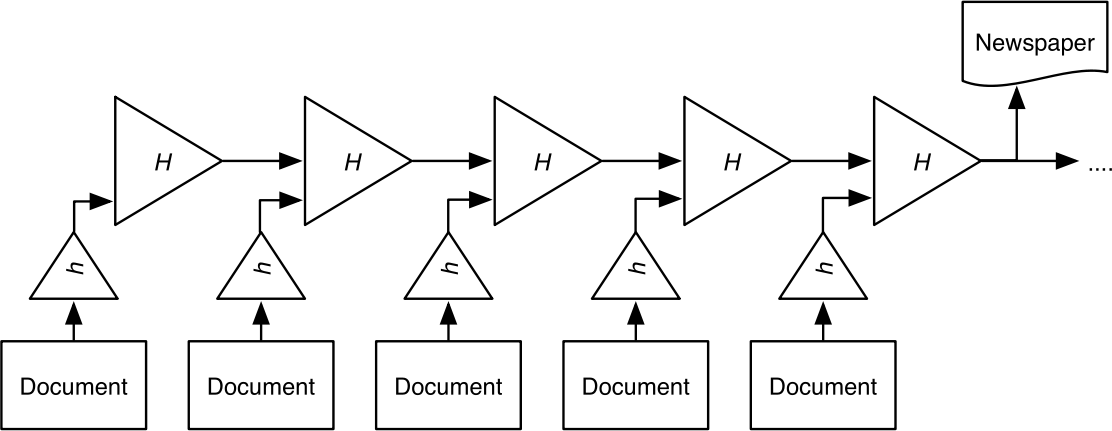
\includegraphics[width=\textwidth]{images/haberstornetta.png}
    \caption{Linking di documenti presso un servizio di timestamp}
    \label{fig:haberstornetta}
\end{figure}
Due possibili scenari possono essere realizzati o combinati:
\begin{enumerate}[1.]
    \item utilizzare un servizio di timestamp (\textit{TTS}) non fidato ma che sia obbligato a produrre timestamp genuini utilizzando il \textit{linking};
    \item distribuire la computazione tra diversi utenti del servizio (\textit{decentralizzazione}).
\end{enumerate}
Tramite \textit{linking} gli hash dei documenti presentati al servizio sono collegati come in Figura \ref{fig:haberstornetta} e il risultato finale è reso pubblico agli utenti. La seconda soluzione prevede che alcuni utenti, scelti randomicamente, producano il timestamp dell'hash in modo tale da non centralizzare il servizio.\newline
Una implementazione della blockchain di Haber e Stornetta è attiva dal 1995: l'azienda \textit{Surety}\footnote{\href{http://surety.com}{Surety}} ogni settimana pubblica una stringa in \textit{base 16} dell'hash di tutte le nuove signature dei clienti della settimana sulla rivista \textit{New York Times}.
\begin{figure}[H]
    \centering
    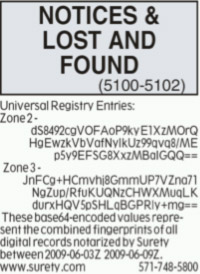
\includegraphics[width=0.35\textwidth]{images/nyt.jpg}
    \caption{Esempio del \textit{base 16} pubblicato sul New York Time da Surety}
    \source{Surety}
\end{figure}

\subsection{Blockchain come sistema di pagamento}
L'implementazione teorica della blockchain di Haber e Stornetta è molto simile a quella presentata nel whitepaper di Satoshi Nakamoto\cite{bitcoin}, infatti, tre degli otto paper citati nel documento \textit{Bitcoin: A Peer-to-Peer Electronic Cash System} sono scritti proprio dai due crittografi\footnote{In quanto l'identità di Satoshi non è mai stata svelata questo fatto ha alimentato voci per cui proprio i due crittografi siano i creatori dei Bitcoin, vedi appendice \ref{app:satoshi}.}.\newline
L'obiettivo di Satoshi era quello di creare un sistema di pagamento elettronico decentralizzato con un forte utilizzo della crittografia, lo stesso che ha portato alla creazione, tra gli anni '90 e 2000, di \textit{eCash}, \textit{SET}, \textit{Bit Gold} e \textit{b-cash}. Tutte queste proposte hanno riscontrato dei problemi per cui non era sicuro metterle in pratica ma hanno dato spunto e suggerimenti a Nakamoto.
L'implementazione di Nakamoto permette di utilizzare la blockchain come infrastruttura per effettuare delle \textit{transazioni} di Bitcoin tra utenti senza necessità di utilizzare terze parti. Gli utenti che intendono utilizzare questa criptomoneta possono convertire, tramite specializzati servizi, la propria valuta in token Bitcoin (\textit{BTC}) secondo il valore in corso della criptomoneta.\newline
I Bitcoin sono soggetti a fluttuazioni di valore come ogni altro mercato; ciò avviene a causa del rapporto domanda e offerta ma anche dal numero di utilizzatori che ripongono la propria fiducia nel protocollo della criptomoneta.
\begin{figure}
    \centering
    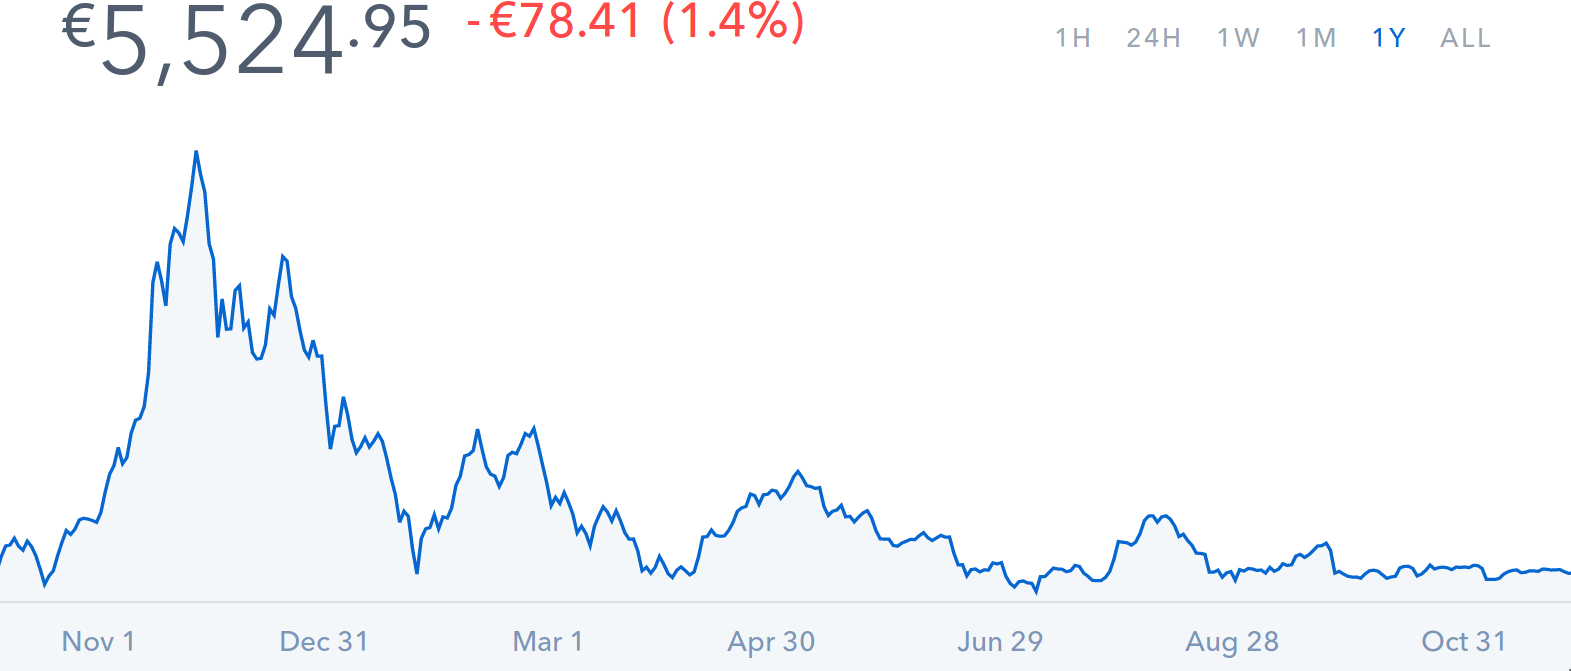
\includegraphics[width=\textwidth]{images/bitcoinchart.png}
    \caption{Andamento del cambio BTC/EUR nell'ultimo anno e valore attuale (Ottobre, 2018). Il picco più alto raggiunto è di circa $17$ mila Euro il 17 Dicembre 2017.}
    \source{coinbase.com}
\end{figure}

\section{Struttura}
Una blockchain è un lista di record, chiamati blocchi, collegati tramite l'utilizzo di tecniche crittografiche che permette solo azioni di inserimento. Ogni record o blocco contiene le informazioni sulle transazioni effettuate tra gli utenti.
In questo modo la lista dei blocchi rappresenta uno storico (registro) di tutti i movimenti che sono stati effettuati e quindi è anche possibile risalire al bilancio totale di ciascun utente.
In quanto non esiste una definizione ed implementazione globalmente valida di blockchain verrà presentata quella utilizzata per i Bitcoin come generica.\newline
Una blockchain è generalmente composta da alcuni elementi fondamentali:
\begin{itemize}
    \item blocco;
    \item data;
    \item rete.
\end{itemize}

\subsection{Blocco}
Un blocco è un singolo elemento della lista formata da tutti i record componenti la blockchain.
\begin{figure}[H]
    \centering
    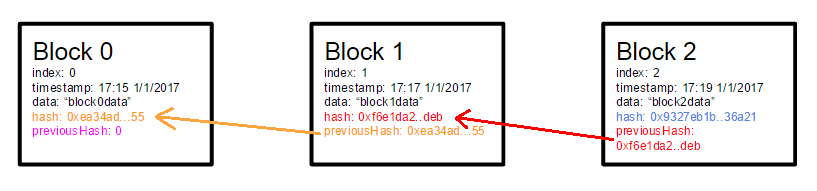
\includegraphics[width=\textwidth]{images/blockchain_basic.png}
    \caption{Esempio di blockchain formata da tre blocchi}
\end{figure}
I blocchi sono connessi come una lista tramite l'utilizzo di funzioni di hashing e quindi, per design, sono resistenti alla modifica dei dati. Ogni blocco è formato da un header, contenente un indice, un timestamp, l'hash del blocco che lo precede nella lista e l'hash dei dati che formano il contenuto del blocco e che devono essere memorizzati permanentemente.\newline
La crittografia fornisce sia autenticazione che verifica ed è usata per garantire un sistema di computazione sicuro senza un singolo proprietario o sistema centrale.\newline
Il primo nodo della lista è chiamato \textbf{genesi} in quanto da questo verrà creata la lista che compone la blockchain. Nella maggior parte delle implementazioni questo blocco è inserito nel codice sorgente, non produce o consuma dati e non è collegato a nessun precedente blocco.
\begin{table}[H]
    \caption{Blocco \textit{genesi} della blockchain per i Bitcoin, il timestamp corrisponde alla data di Sabato 3 Gennaio 2009 alle ore 18:15:05}
    \centering
    \resizebox{\textwidth}{!}{\begin{tabular}{|r|l|}
        \hline
        index & 1\\
        timestamp & 1231006505\\
        data & 0x4a5e1e4baab89f3a32518a88c31bc87f618f76673e2cc77ab2127b7afdeda33b\\
        hash & 0x000000000019d6689c085ae165831e934ff763ae46a2a6c172b3f1b60a8ce26f\\
        previousHash & 0000000000000000000000000000000000000000000000000000000000000000\\
        \hline
    \end{tabular}}
\end{table}
Il blocco successivo a quello di genesi avrà un hash diverso in quanto almeno il timestamp e l'indice del blocco saranno diversi. Il \textit{linking} avviene inserendo l'hash dell'header del blocco precedente nel campo \texttt{previousHash} del nuovo blocco: ogni blocco ha un puntatore al blocco precedente in quanto sono collegati tramite il \texttt{previousHash}.\newline
Procedendo con questo metodo è possibile realizzare una lista di blocchi indefinitamente lunga e che permette di salvare, senza possibilità di modifica, dei dati. Dato un blocco, già inserito nella blockchain, una eventuale modifica dello stesso comporta la necessità di modificare tutti i blocchi che lo succedono al fine di avere un lista integra con il linking degli hash.\newline
Modificando un blocco $x$ con indice $x_i$ in una blockchain di lunghezza $l$ (con $l\ge x_i$) significa modificare l'hash $h(x)$ e quindi dover aggiornare tutti i \texttt{previousHash} dei blocchi $\{x_{i+1},\dots,x_l\}$. Di conseguenza la difficoltà nell'eseguire questa operazione è direttamente proporzionale al numero dei blocchi da aggiornare, a differenza della modifica di un singolo elemento in una normale lista.\newline
In aggiunta, al fine di rendere più computazionalmente difficile la modifica dei singoli blocchi è stato introdotto un valore, \textit{nonce}, che deve essere calcolato ed inserito nell'header di ogni nuovo blocco affinchè venga considerato valido e possa essere inserito nella lista. Questo è possibile grazie ad una proprietà delle funzioni di hashing chiamata \textit{puzzle friendliness}: per inserire un blocco nella lista è necessario trovare un nonce che rispetti determinate tempistiche e parametri imposti dalla blockchain stessa. Affinchè un blocco sia considerato valido deve essere trovato un valore $x$ tale che $h(x||k)$ abbia determinate caratteristiche.\newline
Genericamente, risolvere un \textit{puzzle} tramite funzioni di hashing, significa trovare un valore $x$ tale per cui $h(x||k)\in Y$ con $k$ scelto in una distribuzione ad alta entropia minima e $Y$ l'insieme dei valori di output accettabili.\footnote{L'entropia minima è data dai bit del risultato prodotto nell'evento a minor probabilità ed è calcolata come $-log_2(p)$. Una distribuzione ad altra entropia minima significa che la possibilità che si verifichi un evento sia molto bassa ma equalmente possibile.}\newline
Nel caso della blockchain per i Bitcoin si tratta di un puzzle di ricerca di un valore $x$ tale per cui $h(k||x)<T$ con $T$ il valore del target fissato come un numero a $256$ bit e $k$ l'hash dell'header blocco.\newline
Una volta trovato un valore di $x$ valido, allora il blocco è accettato ed è aggiunto alla lista. Il valore di $x$ è un numero a $32$ bit che per le proprietà delle funzioni di hashing non risulta possibile prevedere o calcolare efficientemente per la proprietà della resistenza alla preimmagine.\newline
Il target $T$ attuale (Ottobre 2018) è:
\begin{equation}
    000000000000000000272fbd0000000000000000000000000000000000000000
\end{equation}
quindi per aggiungere un nuovo blocco alla lista è necessario che $h(x||k)$ sia un valore minore di $T$. Al diminuire del valore di $T$ aumenta la complessità per la ricerca di $x$.\newline
In decimale il valore del target è:
\begin{equation}
    3753318892370425056811838111019504329853891761930240000
\end{equation}
Una volta inserito un nuovo blocco nella blockchain risulta evidente che la difficoltà nel validarlo è molto bassa grazie alle proprietà delle funzioni di hashing: la computazione di un hash deve essere efficiente e deterministica.\newline
Partendo, infatti, dal blocco genesi è possibile calcolare in maniera efficiente tutti gli hash dei blocchi successivi e controllare che l'hash prodotto corrisponda con quello riportato dal blocco successivo come \texttt{previousHash} e che il \textit{nonce} trovato abbia prodotto un valore accettabile.\newline
Al fine di ottimizzare questo tipo di calcolo è possibile evitare di partire dal blocco di indice $0$ e dare per assodato che i primi $x$ blocchi, con $x$ considerato sicuro, siano validi.
\begin{figure}[H]
    \centering
    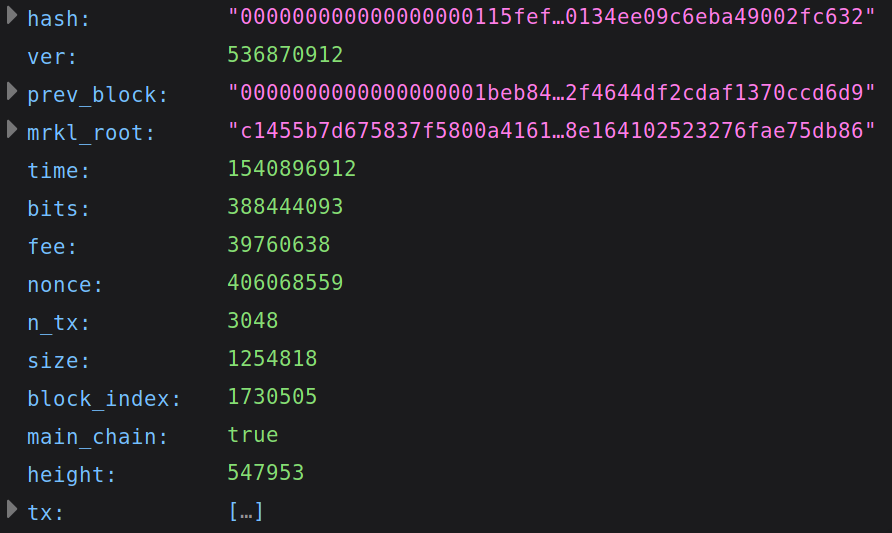
\includegraphics[width=\textwidth]{images/block.png}
    \caption{Struttura del blocco $547953$ in formato chiave/valore.}
\end{figure}

\subsection{Data}
L'obiettivo della blockchain è permettere che delle informazioni vengano salvate all'interno dei blocchi permanentemente e senza possibilità di modifica se non con un aggiornamento successivo referenziato in nuovo blocco (storicità del dato).\newline
Nel caso dei Bitcoin i dati fondamentali salvati all'interno dei blocchi riguardano le \textbf{transazioni} che sono avvenute tra i vari utilizzatori; in questo modo è possibile creare una storicizzazione dei vari scambi e conoscere gli effettivi saldi di ciascun utente.\newline
Al contrario dei classici sistemi bancari o di alcune blockchain come Ethereum\cite{ethereumwhite}, Bitcoin utilizza un modello di tracciamento degli asset non consumati chiamati \textit{unspent transaction output} (\textbf{UTXO}): il bilancio di un utente corrisponde al totale delle transazioni ricevute nel corso della progressione della blockchain e non esiste un ammontare aggiornato ad ogni movimento.\newline
Un utente può effettuare una transazione di $x$ BTC soltanto se il totale $t$ delle transazioni \textit{UTXO} è sufficiente da coprire la spesa; nel caso in cui $x$ sia minore del bilancio totale allora vengono create due transazioni in quanto una UTXO non è spendibile due volte:
\begin{itemize}
    \item una transazione di $x$ BTC verso il destinatario
    \item una transazione UTXO di ritorno di $t-x$
\end{itemize}
La seconda transazione è detta di \textit{cambio} in quanto dalla transazione UTXO di partenza è necessario rimuovere i $x$ BTC spesi; in questo modo, assieme alle altre accumulate, andrà a diminuire il valore totale del conto dell'utente.\newline
Affinchè una transazione possa essere considerata valida deve essere stata inserita in un blocco all'interno della blockchain; per garantire maggiore sicurezza è possibile definire un minimo di 6 \textit{conferme}\footnote{Una transazione inserita nell'ultimo blocco della blockchain ha una sola conferma; ogni blocco aggiunto alla blockchain incrementa il numero di conferme e l'infattibilità di un attaccante di portare attacchi.}. Ogni transazione è composta da almeno un input ed un output. Ogni input implica un movimento di valuta da un output di una transazione precedente (UTXO), gli output sono visti come depositi in attesa che una transazione in input li spenda. Infatti, in totale degli asset posseduti da un utente è la somma degli output delle transazioni ricevute all'interno della blockchain.
\begin{figure}
    \centering
    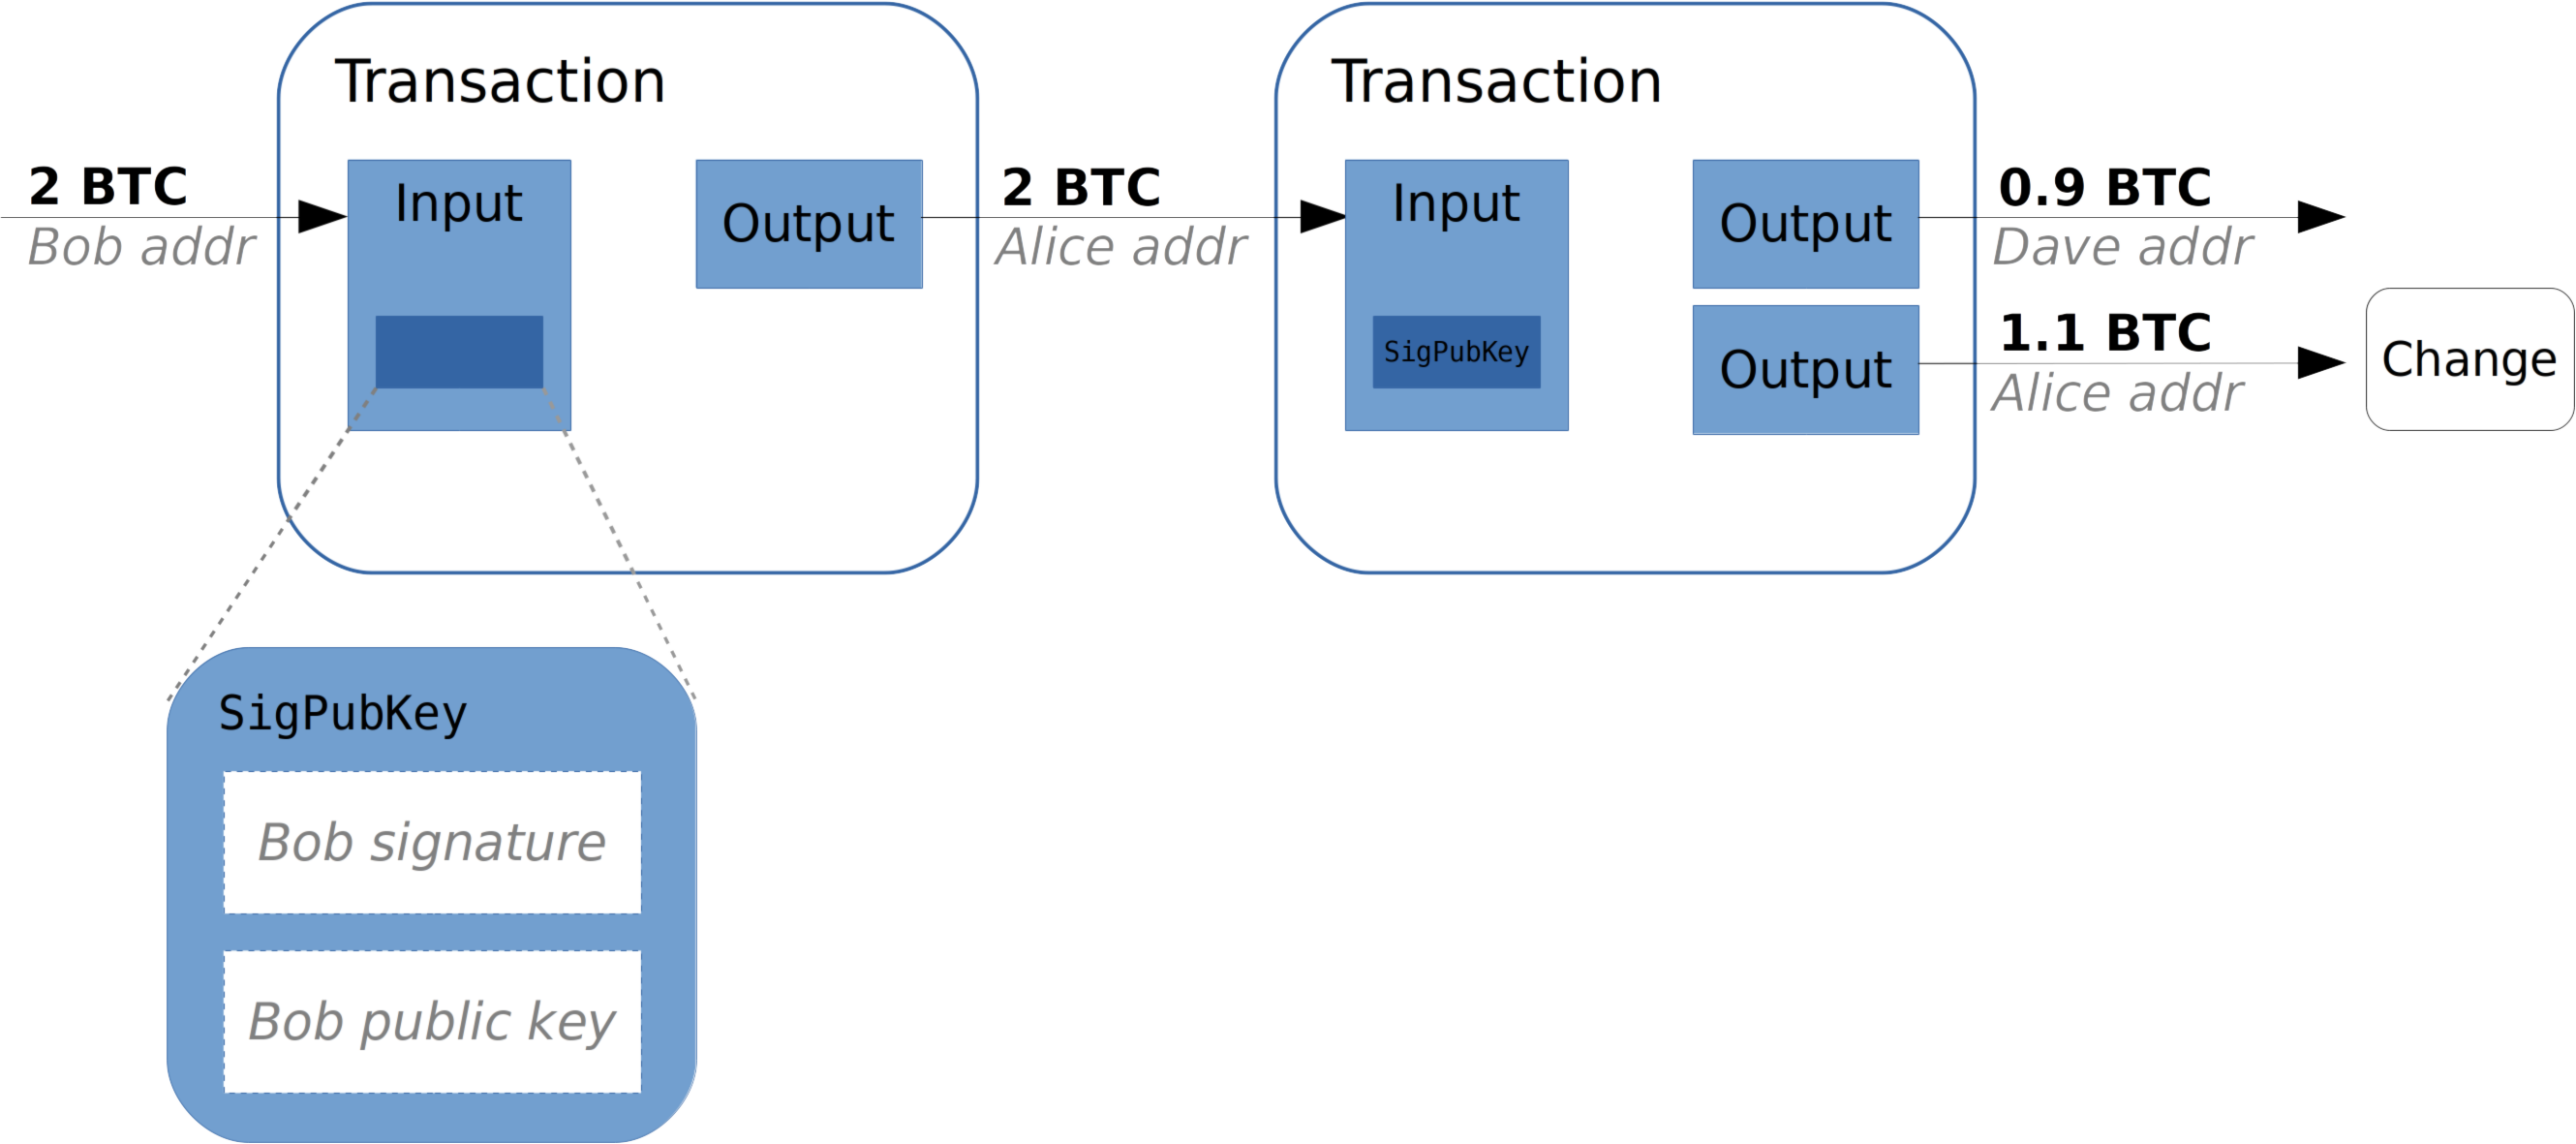
\includegraphics[width=\textwidth]{./images/tx-schema.png}
    \caption{Esempio di due transazioni tra Bob, Alice e Dave.}
\end{figure}
Per poter inviare o ricevere valuta digitale è necessario che le parti creino le coppie di chiavi asimmetriche e quindi abbiano un \textbf{wallet}: solitamente si tratta di un software che permette di creare, salvare le chiavi private e condividere le chiavi pubbliche dell'utente.\newline
I wallet forniscono delle funzionalità ad alto livello per poter effettuare transazioni facilmente e tener traccia del saldo dell'utente analizzando tutta la blockchain alla ricerca di transazioni UTXO che sono associate alla chiave pubblica dell'utente e quindi utilizzabili.\newline
Una volta che le parti hanno accesso ai wallet e quindi alle proprie chiavi, è necessario che si condividano gli indirizzi per poter ricevere denaro; l'indirizzo del wallet corrisponde alla digital signature della chiave pubblica dell'utente in formato base 58.\newline
Un indirizzo di esempio è:
\begin{center}
    \texttt{1A1zP1eP5QGefi2DMPTfTL5SLmv7DivfNa}
\end{center}
questo indirizzo è associato al blocco di genesi ed è stato il primo a ricevere Bitcoin\footnote{L'indirizzo molto probabilmente appartiene a Satoshi Nakamoto}.\newline
Utilizzando gli indirizzi ed i wallet non è necessario l'uso di un sistema centrale che generi o associ delle identità agli utenti ma è possibile creare una chiave pubblica ogni volta che lo si ritiene necessario (virtualmente per ogni transazione).\newline
Una volta creati gli indirizzi per poter ricevere Bitcoin è necessario comunicare il proprio indirizzo; per le proprietà delle funzioni di hashing saranno univoci e sicuri (è computazionalmente inefficiente riuscire a calcolare la chiave privata). Una volta che una parte ha ricevuto l'indirizzo del destinatario è possibile creare una transazione che, se aggiunta ad un blocco inserito nella blockchain, permetterà all'utente di utilizzare l'output di quella transazione come input per altri movimenti.\newline
Al fine di garantire che esclusivamente il destinatario della transazione possa accedere ai fondi inviati è fondamentale che nella transazione venga inserito uno script di controllo: chi possiede la chiave privata associata alla pubblica utilizzata nella transazione può utilizzare l'output di quella transazione.

\subsubsection{Transazioni P2PKH}\label{sec:transazione}
Una transazione \textbf{P2PKH} (\textit{Pay-2-Public-Key Hash}) è la modalità più comune di trasferimento di denaro all'interno della rete Bitcoin.
Una transazione è un insieme di byte che vengono pubblicati nella rete \textit{p2p} e affinchè possa essere accettata è necessario che il blocco in cui viene inserita sia valido e inserito nella blockchain.
Ogni transazione è composta da almeno un input ed un output; gli input derivano da transazioni \textit{UTXO} dell'utente che vuole effettuare l'operazione; gli output verranno trattati come transazioni UTXO dell'utente destinatario.\newline
L'aggiunta di un blocco alla blockchain risulta essere molto dispendiosa e, quindi, non è efficiente utilizzare un blocco per ogni operazione ma ogni blocco raccoglie diverse transazioni (in media 2000). Per una facile gestione del blocco e della sua validazione le transazioni vengono salvate in una struttura dati chiamata \textbf{Merkle Tree} all'interno del blocco e solo l'hash della radice dell'albero viene salvato nell'header.\newline
La struttura \textit{Merkle Tree} sfrutta le funzioni di hashing per creare un albero binario contenente tutte le transazioni del blocco.\newline
L'albero è costruito partendo dalle foglie: le transazioni, inserite nel blocco in ordine di arrivo, sono raggruppate in coppie e per ogni gruppo ne viene calcolato l'hash. Gli hash creati costituiscono il nuovo livello dell'albero che a loro volta vengono divisi in gruppi di due e, calcolati i rispettivi hash, formeranno il livello successivo.
Le operazioni vengono ripetute finchè non si ottiene un singolo hash come radice dell'albero.\newline
\begin{figure}
    \centering
    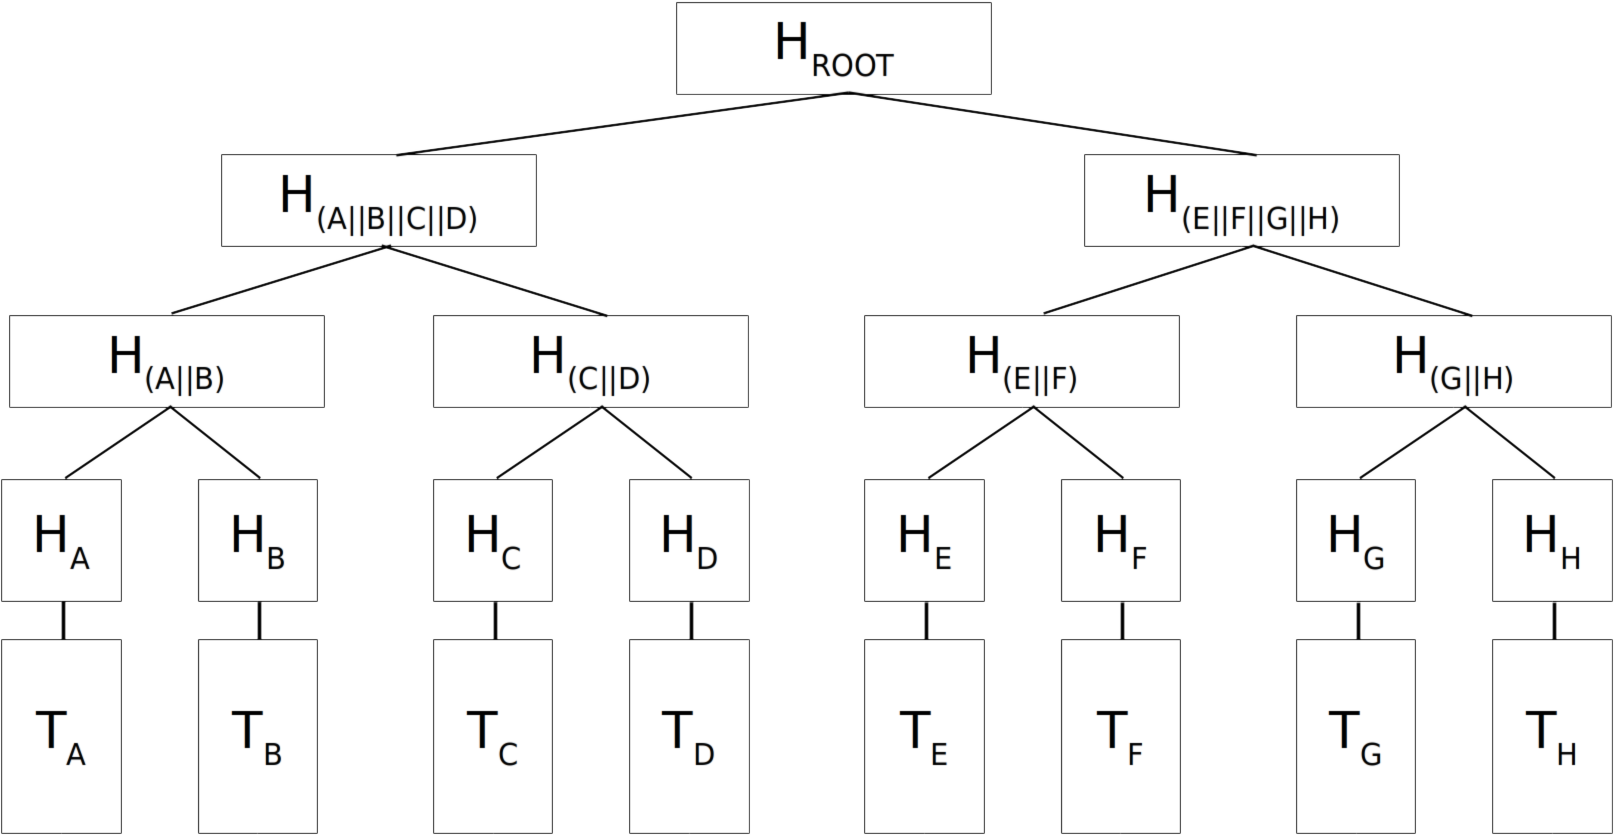
\includegraphics[width=0.9\textwidth]{./images/merkle.png}
    \caption{In un albero \textit{Merkle} i blocchi di dati sono raggrupati in coppie e l'hash di ciascuno è salvato nel nodo padre. I nodi padre sono valutati in coppie e i loro hash sono salvati nel livello dell'albero superiore fino alla radice.}
    \label{fig:merkle}
\end{figure}
In questo modo si ha la certezza che i dati non vengano cambiati: non è possibile cambiare una transazione una volta resa pubblica in quanto è necessario aggiornare l'albero di Merkle e quindi l'header del blocco.
Un altro vantaggio dato dalla struttura dati ad albero è l'efficienza nel provare che una transazione appartenga a quel blocco e quindi al Merkle Tree: dati $n$ nodi in un albero è necessario conoscere $log(n)$ valori per poter provare la presenza di una transazione.\newline
Per dimostrare, ad esempio, la presenza della transazione $T_C$ nella Figura \ref{fig:merkle} è sufficiente conoscere $T_C$, $H_{(C||D)}$ e $H_{(A||B||C||D)}$; in questo modo in tempo  $log(n)$ è possibile calcolare e validare i singoli hash.\newline
Ogni transazione $P2PKH$ è composta in diversi passaggi:
\begin{enumerate}[1.]
    \item identificare una precedente transazione che contiene UTXO che l'utente controlla (valuta spendibile);
    \item creare i gli input della nuova transazione referenziando la transazione UTXO;
    \item creare gli output della nuova transazione utilizzando il codice \texttt{scriptPubKey} per crare una transazione UTXO: \textit{locking script};
    \item creare le condizioni di sblocco in base alle condizioni imposte dal precedente \textit{locking script}.
\end{enumerate}
Una transazione è composta da diversi campi che sono di dimensione fissa in modo tale che sia facile comprenderne le caratteristiche. In particolare è composta da:
\begin{itemize}
    \item numero di versione: per distinguere eventuali modifiche nel protocollo
    \item input della transazione; se le condizioni dell'output della transazione UTXO sono valide allora è possibile spenderlo
        \begin{itemize}
            \item numero delle transazioni UTXO consumate (è possibile utilizzare diverse UTXO)
            \item puntatore alle transazioni precedenti che possono essere consumate
            \item indice dell'output della precedenti transazioni UTXO
        \end{itemize}
    \item script di sblocco \texttt{scriptSig}: signature dell'utente che crea la transazione (mittente) e la chiave pubblica dell'utente che riceve i Bitcoin
    \item numero di sequenza
    \item output della transazione
        \begin{itemize}
            \item numero degli output
            \item ammontare dell'output consumato
            \item lo script di \textit{locking} o \texttt{scriptPubKey}: definisce le condizioni per cui l'output può essere consumato (solo l'utente con la signature corretta può accedere ai fondi)
        \end{itemize}
\end{itemize}
\begin{figure}
    \centering
    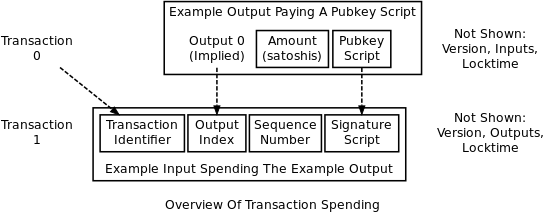
\includegraphics[width=\textwidth]{./images/example-tx.png}
    \caption{L'utente crea una transazione $1$ utilizzando gli output non spesi della transazione $0$.}
    \source{bitcoin.org}
\end{figure}
Un esempio di transazione in formato esadecimale è:
\begin{table}[H]
    \begin{tabular}{l}
        \texttt{01000000019c2e0f24a03e72002a96acedb12a632e72b6b74c05dc3ceab1fe78237f886c48}\\
        \texttt{010000006a47304402203da9d487be5302a6d69e02a861acff1da472885e43d7528ed9b1b5}\\
        \texttt{37a8e2cac9022002d1bca03a1e9715a99971bafe3b1852b7a4f0168281cbd27a220380a01b}\\
        \texttt{3307012102c9950c622494c2e9ff5a003e33b690fe4832477d32c2d256c67eab8bf613b34e}\\
        \texttt{ffffffff02b6f50500000000001976a914bdf63990d6dc33d705b756e13dd135466c06b3b5}\\
        \texttt{88ac845e0201000000001976a9145fb0e9755a3424efd2ba0587d20b1e98ee29814a88ac00}\\
        \texttt{000000}
    \end{tabular}
\end{table}
Questo è il formato che verrano utilizzato come rappresentazione della transazione all'interno del blocco e quindi all'interno del \textit{Merkle Tree}.
\begin{figure}[H]
    \centering
    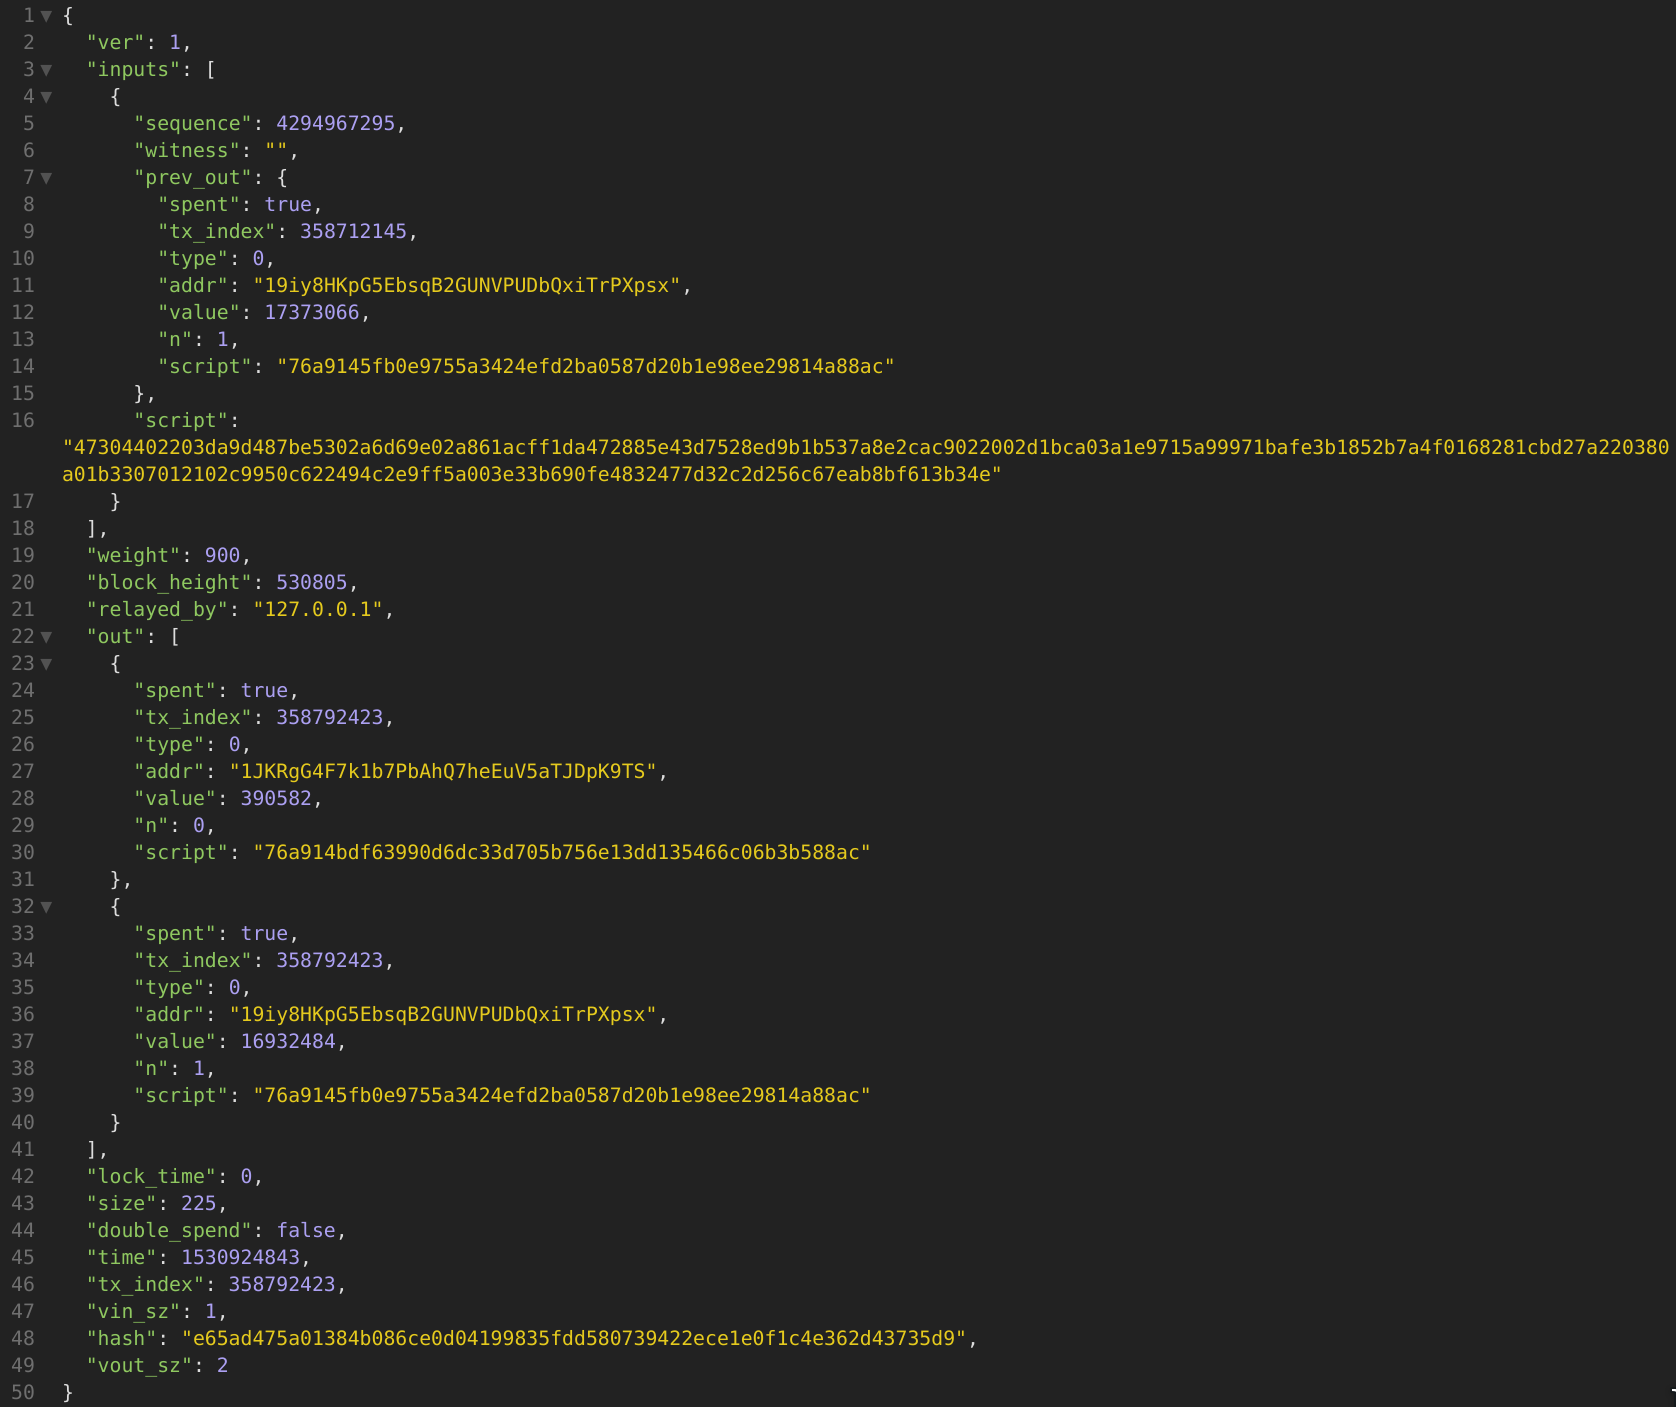
\includegraphics[width=\textwidth]{./images/tx.png}
    \caption{Struttura di una transazione di $0.00390582$ BTC.}
    \label{fig:tx}
\end{figure}
Dalla Figura \ref{fig:tx} è possibile vedere che la transazione presa in esame ha:
\begin{itemize}
    \item un input:
        \begin{itemize}
            \item una \textit{UTXO} dell'indirizzo \texttt{19iy8HKpG5EbsqB2GUNVPUDbQxiTrPXpsx} con un valore di $17373066$ Satoshi ($0.17373066$ BTC);
        \end{itemize}
    \item due output
        \begin{itemize}
            \item uno destinato a diventare una UTXO per l'indirizzo\\\texttt{1JKRgG4F7k1b7PbAhQ7heEuV5aTJDpK9TS} con un valore di $390582$ Satoshi ($0.00390582$ BTC)
            \item l'altro è dato da una transazione di \textit{cambio} verso l'indirizzo sorgente per generare una UTXO con i Satoshi non spesi ($16932484$ Satoshi, $0.16932484$ BTC).
        \end{itemize}
\end{itemize}
La differenza tra il totale in input ed in output è stata spesa come \textit{fee} (tassa) per aggiungere la transazione al blocco ed essere validata dalla rete.\newline
Lo script di \textit{locking} o \texttt{scriptPubKey} è del codice espresso come \texttt{Bitcoin~Script}: un linguaggio Turing-incompleto stateless basato su stack che permette di eseguire alcune operazioni base sulle transazioni tramite diversi \texttt{OP\_CODES}.\newline
Affinchè la transazione abbia successo è necessario che gli script di \textit{locking} e di sblocco eseguano correttamente:
\begin{table}[H]
    \centering
    \begin{tabular}{l|l|l}
        Locking Script & Unlocking Script & Script\\
        \hline
        \texttt{OP\_DUP}         & \texttt{<signature>} & \texttt{<signature>}\\
        \texttt{OP\_HASH160}     & \texttt{<publicKey>} & \texttt{<publicKey>}\\
        \texttt{<pubKeyHash?>}   &                      & \texttt{OP\_DUP}\\
        \texttt{OP\_EQUALVERIFY} &                      & \texttt{OP\_HASH160}\\
        \texttt{OP\_CHECKSIG}    &                      & \texttt{<pubKeyHash?>}\\
                                 &                      & \texttt{OP\_HASH160}\\
                                 &                      & \texttt{<pubKeyHash?>}\\
    \end{tabular}
\end{table}
Essendo una architettura basata su stack le operazioni da eseguire e i dati utilizzano una struttura dati in cui sono inseriti e rimossi in ordine \textit{First-In-First-Out}.\newline
L'esecuzione dello script avviene tramite alcuni passaggi:
\begin{table}[H]
    \centering
    \begin{tabular}{p{3cm}|p{7.7cm}|p{3cm}}
        Script & Stack & Eseguite\\
        \hline
        \texttt{\textbf{<signature>}} & &\\
        \texttt{<publicKey>}          & &\\
        \texttt{OP\_DUP}              & &\\
        \texttt{OP\_HASH160}          & &\\
        \texttt{<pubKeyHash?>}        & &\\
        \texttt{OP\_EQUALVERIFY}      & &\\
        \texttt{OP\_CHECKSIG}         & 304402203da9\dots281cbd27a220380a01b330701 & \\
    \end{tabular}
    \caption{La signature del mittente della transazione è inserita nello stack}
\end{table}

\begin{table}[H]
    \centering
    \begin{tabular}{p{3cm}|p{7.7cm}|p{3cm}}
        Script & Stack & Eseguite\\
        \hline
        \texttt{<signature>}          & &\\
        \texttt{\textbf{<publicKey>}} & &\\
        \texttt{OP\_DUP}              & &\\
        \texttt{OP\_HASH160}          & &\\
        \texttt{<pubKeyHash?>}        & &\\
        \texttt{OP\_EQUALVERIFY}      & 02c9950c6224\dots7d32c2d256c67eab8bf613b34 &\\
        \texttt{OP\_CHECKSIG}         & 304402203da9\dots281cbd27a220380a01b330701 & \texttt{<signature>}\\
    \end{tabular}
    \caption{La chiave pubblica del mittente della transazione è inserita nello stack; \texttt{scriptPubkey} è stato caricato.}
\end{table}

\begin{table}[H]
    \centering
    \begin{tabular}{p{3cm}|p{7.7cm}|p{3cm}}
        Script & Stack & Eseguite\\
        \hline
        \texttt{<signature>}          & &\\
        \texttt{<publicKey>}          & &\\
        \texttt{\textbf{OP\_DUP}}     & &\\
        \texttt{OP\_HASH160}          & &\\
        \texttt{<pubKeyHash?>}        & 02c9950c6224\dots7d32c2d256c67eab8bf613b34 &\\
        \texttt{OP\_EQUALVERIFY}      & 02c9950c6224\dots7d32c2d256c67eab8bf613b34 & \texttt{<publicKey>}\\
        \texttt{OP\_CHECKSIG}         & 304402203da9\dots281cbd27a220380a01b330701 & \texttt{<signature>}\\
    \end{tabular}
    \caption{\texttt{OP\_DUP} duplica la testa dello stack: l'operazione è necessaria per eseguire prima l'hash della chiave e poi infine il controllo.}
\end{table}

\begin{table}[H]
    \centering
    \begin{tabular}{p{3cm}|p{7.7cm}|p{3cm}}
        Script & Stack & Eseguite\\
        \hline
        \texttt{<signature>}          & &\\
        \texttt{<publicKey>}          & &\\
        \texttt{OP\_DUP}              & &\\
        \texttt{\textbf{OP\_HASH160}} & &\\
        \texttt{<pubKeyHash?>}        &                                            & \texttt{OP\_DUP}\\
        \texttt{OP\_EQUALVERIFY}      & 02c9950c6224\dots7d32c2d256c67eab8bf613b34 & \texttt{<publicKey>}\\
        \texttt{OP\_CHECKSIG}         & 304402203da9\dots281cbd27a220380a01b330701 & \texttt{<signature>}\\
    \end{tabular}
    \caption{\texttt{OP\_HASH160} rimuove il primo elemento dello stack per eseguire prima un'operazione di SHA256 e poi \texttt{RIPEMD-160} sul valore rimosso. Il \textit{RIPEMD} è un algoritmo crittografico di hashing ideato da Hans Dobbertin, Antoon Bosselaers e Bart Preneel  e pubblicato per la prima volta nel 1994. Il \textit{RIPEMD} nacque come alternativa europea alle funzioni \textit{MD4} e \textit{MD5}. Satoshi scelse questo algoritmo in quanto la ridotta lunghezza dell'output garantisce comunque ottimi valori di unicità e quindi resistenza alle collisioni.}
\end{table}

\begin{table}[H]
    \centering
    \begin{tabular}{p{3cm}|p{7.7cm}|p{3cm}}
        Script & Stack & Eseguite\\
        \hline
        \texttt{<signature>}            & &\\
        \texttt{<publicKey>}            & &\\
        \texttt{OP\_DUP}                & &\\
        \texttt{\textbf{OP\_HASH160}}   & &\\
        \texttt{<pubKeyHash?>}          & bdf63990d6dc\dots705b756e13dd135466c06b3b5 & \texttt{OP\_DUP}\\
        \texttt{OP\_EQUALVERIFY}        & 02c9950c6224\dots7d32c2d256c67eab8bf613b34 & \texttt{<publicKey>}\\
        \texttt{OP\_CHECKSIG}           & 304402203da9\dots281cbd27a220380a01b330701 & \texttt{<signature>}\\
    \end{tabular}
    \caption{\texttt{OP\_HASH160} dopo aver eseguito inserisce il risultato nello stack.}
\end{table}

\begin{table}[H]
    \centering
    \begin{tabular}{p{3cm}|p{7.7cm}|p{3cm}}
        Script & Stack & Eseguite\\
        \hline
        \texttt{<signature>}            & &\\
        \texttt{<publicKey>}            & &\\
        \texttt{OP\_DUP}                & &\\
        \texttt{OP\_HASH160}            & bdf63990d6dc\dots705b756e13dd135466c06b3b5 & \texttt{OP\_HASH160}\\
        \texttt{\textbf{<pubKeyHash?>}} & bdf63990d6dc\dots705b756e13dd135466c06b3b5 & \texttt{OP\_DUP}\\
        \texttt{OP\_EQUALVERIFY}        & 02c9950c6224\dots7d32c2d256c67eab8bf613b34 & \texttt{<publicKey>}\\
        \texttt{OP\_CHECKSIG}           & 304402203da9\dots281cbd27a220380a01b330701 & \texttt{<signature>}\\
    \end{tabular}
    \caption{Viene inserito nello stack l'hash della chiave pubblica.}
\end{table}

\begin{table}[H]
    \centering
    \begin{tabular}{p{3cm}|p{7.7cm}|p{3cm}}
        Script & Stack & Eseguite\\
        \hline
        \texttt{<signature>}              & &\\
        \texttt{<publicKey>}              & &\\
        \texttt{OP\_DUP}                  &                                            & \texttt{<pubKeyHash?>}\\
        \texttt{OP\_HASH160}              &                                            & \texttt{OP\_HASH160}\\
        \texttt{<pubKeyHash?>}            &                                            & \texttt{OP\_DUP}\\
        \texttt{\textbf{OP\_EQUALVERIFY}} & 02c9950c6224\dots7d32c2d256c67eab8bf613b34 & \texttt{<publicKey>}\\
        \texttt{OP\_CHECKSIG}             & 304402203da9\dots281cbd27a220380a01b330701 & \texttt{<signature>}\\
    \end{tabular}
    \caption{\texttt{OP\_EQUALVERIFY} prende i due elementi in testi allo stack e se non sono uguali termina l'esecuzione dello script in quanto la transazione non è valida e l'utente non può accedere a quella transazione. L'operazione è composta da due sotto istruzioni: \texttt{OP\_EQUAL} e \texttt{OP\_VERIFY}; la prima inserisce il valore \texttt{True} se i due elementi in cima allo stac sono uguali, la seconda segna la transazione come valida se l'elemento in testa allo stack è \texttt{True}.}
\end{table}

\begin{table}[H]
    \centering
    \begin{tabular}{p{3cm}|p{7.7cm}|p{3cm}}
        Script & Stack & Eseguite\\
        \hline
        \texttt{<signature>}              &      &\\
        \texttt{<publicKey>}              &      & \texttt{OP\_EQUALVERIFY}\\
        \texttt{OP\_DUP}                  &      & \texttt{<pubKeyHash?>}\\
        \texttt{OP\_HASH160}              &      & \texttt{OP\_HASH160}\\
        \texttt{<pubKeyHash?>}            &      & \texttt{OP\_DUP}\\
        \texttt{OP\_EQUALVERIFY}          &      & \texttt{<publicKey>}\\
        \texttt{\textbf{OP\_CHECKSIG}}    & True & \texttt{<signature>}\\
    \end{tabular}
    \caption{\texttt{OP\_CHECKSIG} prende due elementi dallo stack e controlla che la signature della transazione sia valida utilizzando l'hash della chiave pubblica: se è valida allora la transazione può procedere e nello stack viene posizionato il valore \texttt{True}.}
\end{table}

\subsubsection{Transazioni coinbase}
\begin{figure}[H]
    \centering
    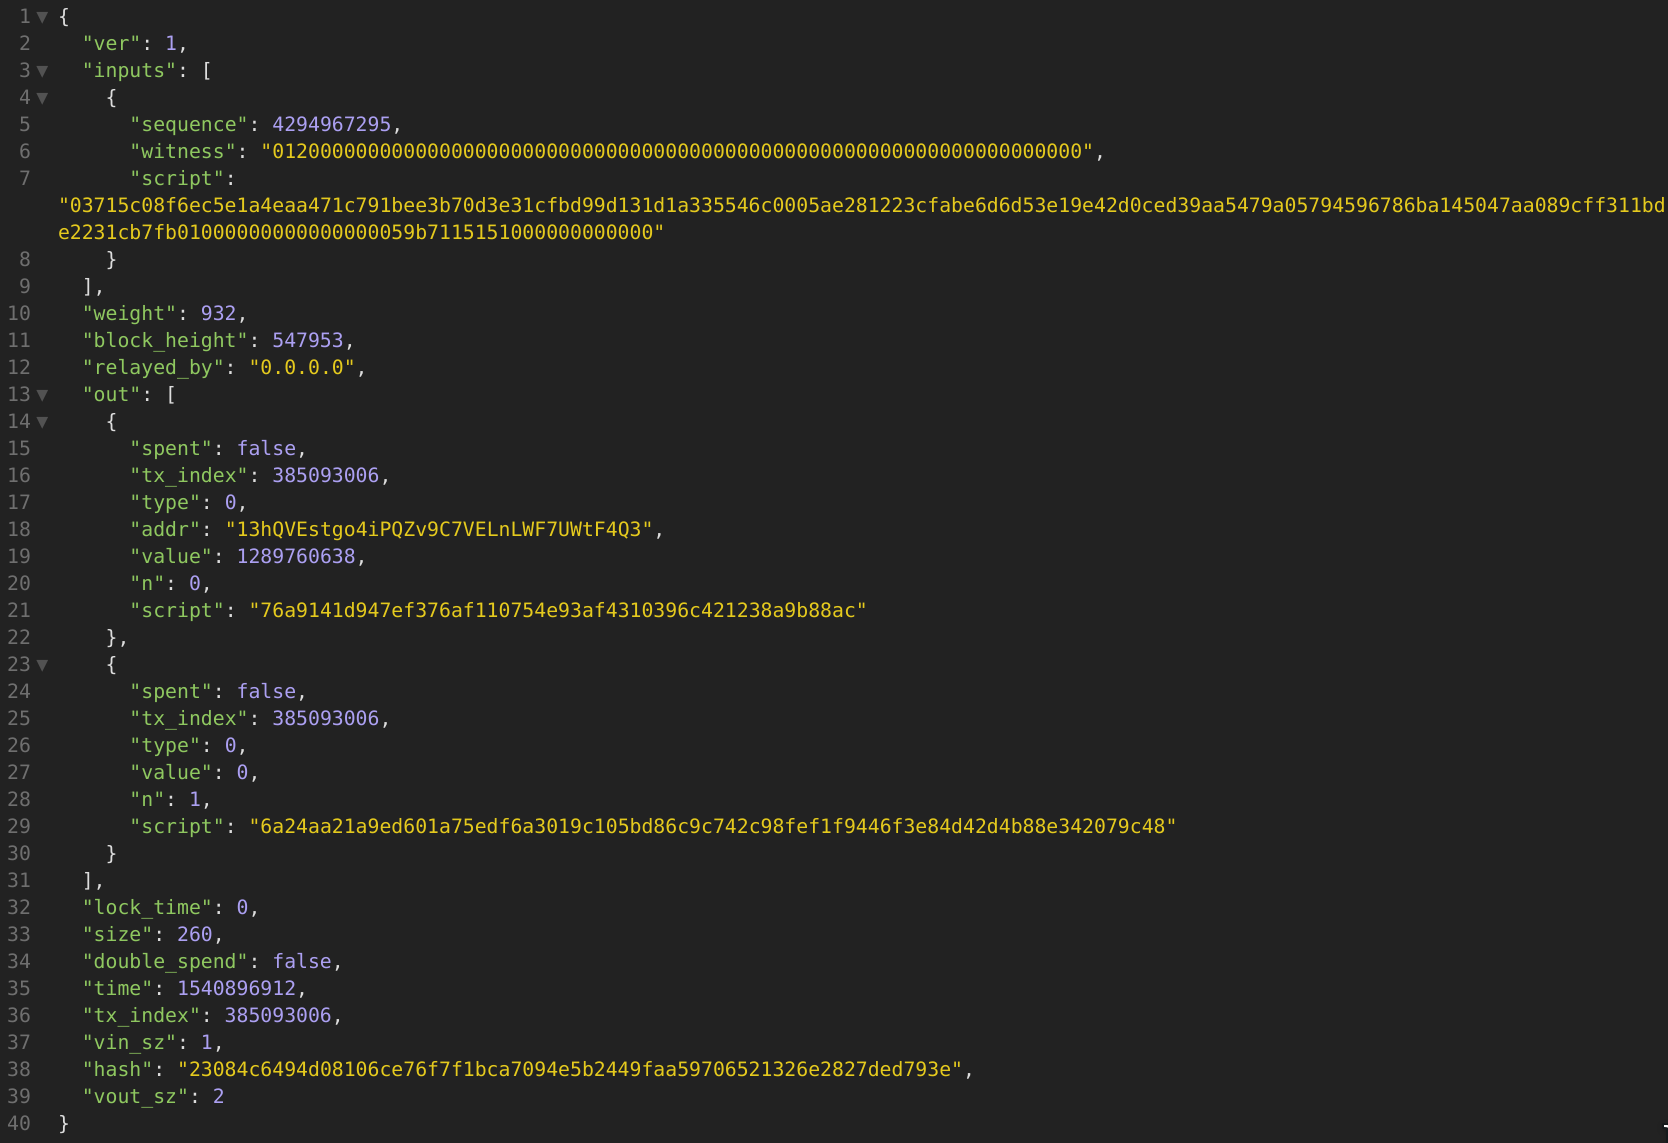
\includegraphics[width=\textwidth]{images/coinbasetx.png}
    \caption{Transazione coinbase per il blocco 547955 di $12.89760638$ BTC all'indirizzo \texttt{13hQVEstgo4iPQZv9C7VELnLWF7UWtF4Q3}.}
\end{figure}
In aggiunta alle transazioni tra utenti con diversi input ed output esistono alcune transazioni che non sono associate a nessuna precedente UTXO e hanno un solo input ed un solo output, queste transazioni sono chiamate \textbf{coinbase}.\newline
Le transazioni coinbase producono nuova valuta: sono formate dalla ricompensa dell'inserimento del blocco nella blockchain con relativa validazione e il totale delle \textit{fee} di ciascuna transazione inserita nel blocco. Ogni blocco quindi ha, quindi, almeno una transazione ed è la prima che viene inserita nell'albero binari di Merkle.\newline
Le transazioni coinbase hanno un formato diverso da quelle tradizionali in quanto hanno un solo input ed output, l'input è un puntatore nulla in quanto non è collegato a nessuna transazione precedente, il valore dell'output è di $12.5$ BTC più le \textit{fee} per ogni transazione inserita ed un parametro "coinbase" arbitrario in cui è possibile inserire qualsiasi tipo di dato. Non è presente nessun \texttt{scriptSig} per l'input in quanto non è necessario sbloccare nessuna transazione precedente.\newline
Inizialmente le transazioni \textit{coinbase} avevano un valore di $50$ BTC ma per evitare un rapido esaurimento dei $21$ milioni di Bitcoin pensati da Nakamoto, è stato implementato un contatore che ogni $210000$ blocchi dimezza questo valore (ovvero ogni $4$ anni). Attualmente una transazione coinbase ha un valore di $12.5$ BTC ma è previsto che per la fine di Maggio 2020 varranno $6.25$.\newline
Il blocco di genesi creato da Satoshi contiene infatti un messaggio nel campo \textit{coinbase}\footnote{\href{https://www.blockchain.com/btc/tx/4a5e1e4baab89f3a32518a88c31bc87f618f76673e2cc77ab2127b7afdeda33b?show\_adv=true}{Transazione coinbase per il blocco di genesi.}}.\newline
Il messaggio è decodificato in ASCII è:
\begin{center}
\item \textit{The Times 03/Jan/2009 Chancellor on brink of second bailout for banks}
\end{center}
Il messaggio si riferisce ad un articolo del 3 Gennaio 2009 (giorni di nascita della blockchain) che fa riferimento ad un piano di salvataggio per le banche dopo la crisi economica del $2008$. Il messaggio è stato utilizzato da Satoshi come prova che il blocco fosse stato minato il 3 Gennaio in quanto non poteva conoscere il titolo dell'articolo in anticipo. In aggiunta è chiaramente una critica ed un atto di sfida agli attuali sistemi di pagamento e gestione del denaro.
Un esempio di transazione coinbase in formato esadecimale è:
\begin{table}[H]
    \begin{tabular}{l}
        \texttt{0100000000010100000000000000000000000000000000000000000000000000000}\\
        \texttt{00000000000ffffffff5c03715c08f6ec5e1a4eaa471c791bee3b70d3e31cfbd99d}\\
        \texttt{131d1a335546c0005ae281223cfabe6d6d53e19e42d0ced39aa5479a05794596786}\\
        \texttt{ba145047aa089cff311bde2231cb7fb01000000000000000059b711515100000000}\\
        \texttt{0000ffffffff027e2fe04c000000001976a9141d947ef376af110754e93af431039}\\
        \texttt{6c421238a9b88ac0000000000000000266a24aa21a9ed601a75edf6a3019c105bd8}\\
        \texttt{6c9c742c98fef1f9446f3e84d42d4b88e342079c480120000000000000000000000}\\
        \texttt{000000000000000000000000000000000000000000000000000}
    \end{tabular}
\end{table}

\subsubsection{Transazioni \textit{multi-signature} o \textit{Pay-to-Script Hash}}
In aggiunta alle transazioni tra due parti è anche possibile utilizzare alcune varianti che permettono di includere diverse parti alla stessa transazione; ad esempio, per dividere le responsabilità su un quantativo di Bitcoin in possesso. Queste transazioni sono deete \textit{multi-signature} o \texttt{multisig} e richiedono che più di una chiave privata per autorizzare una transazione Bitcoin. Le transazioni supportato tramite \texttt{multisig} possono essere intraprese con l'approvazione non unilaterale, ovvero anche con $M$-su-$N$ parti la transazione è accettata: l'idea di base è di impedire che una singola parte controlli le transazioni. Le transazioni multi-signature quindi richiedono cooperazione tra le parti; queste parti possono essere persone, organizzazioni, istituzioni o programmi.\newline
Un esempio di scenario per transazioni multi-signature è il seguente: data un'azienda che accetta Bitcoin come metodo di pagamento per i propri servizi è fondamentale, per ragioni di sicurezza, che il wallet non sia accessibile da un singolo impiegato. L'azienda per riscattare i Bitcoin inviati nella transazione dovrà conoscere lo script che ha generato l'hash e che l'esecuzione dello stesso abbia esito positivo.
L'utilizzo del wallet quindi può essere regolamentato tramite l'utilizzo del \texttt{multisig} e l'istruzione \texttt{OP\_CHECKMULTISIG}.\newline
Il template per una transazione \textit{multi-signature} compone l'output script come:
\begin{table}[H]
    \centering
    \begin{tabular}{c|c|c|c|c|c}
        \texttt{<t>} & \texttt{<pubKey 1>} & \dots & \texttt{<pubkKey n>} & \texttt{<n>} & \texttt{OP\_CHECKMULTISIG}
    \end{tabular}
\end{table}
e lo script di input:
\begin{table}[H]
    \caption{\texttt{OP\_0} inserisce $0$ nello stack}
    \centering
    \begin{tabular}{c|c|c|c}
        \texttt{OP\_0} & \texttt{<signature 1>} & \dots & \texttt{<signature t>}
    \end{tabular}
\end{table}
L'istruzione \texttt{OP\_CHECKMULTISIG}\footnote{Nell'implementazione dell'istruzione \texttt{OP\_CHECKMULTISIG} è presente un bug che causa la rimozione dallo stack di un valore aggiuntivo ma che non viene utilizzato. In quanto la risoluzione del bug comporta notevoli costi è normale inserire un elemento nullo in questo tipo di transazioni} richiede $n$ chiavi pubbliche da verificare e un soglia $t$. L'esecuzione è valida se almeno $t$ su $n$ chiavi pubbliche sono valide per la transazione.\newline
L'esecuzione della dell'istruzione avviene tramite una serie di passi:
\begin{enumerate}
    \item un valore è rimosso dallo stack ed interpretato come numero di chiavi pubbliche;
    \item due o più valori sono inseriti nello stack come lista delle chiavi pubbliche;
    \item un valore è rimosso dallo stack come numero delle signature da controllare;
    \item tutte le signature sono rimosse dallo stack;
    \item l'elemento nullo aggiuntivo viene rimosso dallo stack.
\end{enumerate}
Il risultato è la creazione di due liste di chiavi pubbliche e di signature: la verifica comporta il tentativo di validare le signature con le chiavi pubbliche.\newline Per facilitare la verifica della transazione \textit{multi-signature} è possibile utilizzare, anziché l'hash del wallet del destinatario, l'hash dello script Bitcoin che viene eseguito chiamato \textit{Pay-to-Script Hash} (o \textit{P2SH}). \textit{P2SH} delega la fase di autenticazione ad uno script che definisce le condizioni di successo.\\
\begin{table}[H]
    \centering
    \begin{tabular}{c|c|c}
        \texttt{OP\_HASH160} & \texttt{<redemption script hash>} & \texttt{<OP\_EQUAL>}
    \end{tabular}
\end{table}
\begin{table}[H]
    \centering
    \begin{tabular}{c|c|c|c}
        \texttt{<data 1>} & \dots & \texttt{<data n>} & \texttt{<redemption script>}
    \end{tabular}
\end{table}

\subsection{Rete}
La rete Bitcoin è una rete \textit{peer-2-peer} con topologia randomica e senza gerarchie tra i vari nodi ed è la chiave per raggiungere decentralizzazione e consenso distribuito.\newline
Un nodo all'interno della rete peer-2-peer di Bitcoin comunica con gli altri tramite protocollo TCP (porta di default $8883$) per ricevere informazioni e comunicarle agli altri nodi tramite algoritmi di \textit{gossip} [\ref{appendix:gossip}]. In quanto si tratta di una topologia altamente dinamica è necessario che i nodi aggiornino frequentemente la lista degli altri nodi con cui comunicare: ad esempio molti software di wallet considerano un nodo offline quando non ci sono comunicazione per più di tre ore.\newline
La rete Bitcoin è utilizzata per diffondere le transazioni tramite algoritmi di \textit{flooding} per gossip. Ad esempio per una transazione tra Alice e Bob:
\begin{enumerate}
    \item Alice crea la transazione come visto in \ref{sec:transazione};
    \item la transazione viene inoltrata ai peer connessi ad Alice;
        \begin{enumerate}
            \item i peer controllano che lo script sia sintatticamente valido;
            \item i peer controllano che lo script di unlocking sia valido per ogni UTXO;
            \item i peer controllano che l'ammontare della transazione sia spendibile e non già speso in un'altra transazione (per evitare il \textit{double spending});
            \item se la transazione è già conosciuta o i check sono falliti non ci sono successivi inoltri (ogni transazione è univoca ed ha un hash associato) e la transazione viene rifiutata;
            \item altrimenti i peer creano un nuovo blocco e/o aggiungono la transazione al proprio albero Merkle;
        \end{enumerate}
    \item una volta inserita la transazione nel blocco, i peer inoltrano la richiesta agli altri nodi connessi;
\end{enumerate}
In quanto si tratta di una rete peer-2-peer è possibile che ci siano delle latenze e che l'ordine delle transazioni non sia lo stesso con cui sono state pubblicate o che si creino situazioni di \textit{race condition}: nel caso Alice voglia tentare di inviare lo stesso ammontare di Bitcoin a Bob e Charlie (double spending) solamente la prima transazione che verrà inserita nel blocco e successivamente nella blockchain sarà accettata; tutte gli altri peer che avranno aggiunto nel loro albero di transazioni l'altra transazione la elimineranno in quanto ritenuta invalida.\newline
L'assenza di una struttura nelle reti \textit{p2p} ne facilita la gestione ma al costo non ottimale per la distribuzione dei messaggi: non è possibile prevedere ad esempio gli esatti destinatari di un messaggio senza incorrere un ripetizioni.\newline
In una rete non strutturata i collegamenti tra i nodi sono effettuati arbitrariamente e localmente (di \textit{peer} in \textit{peer}).\newline
Al fine di garantire che tutti i \textit{peer} ricevano il messaggio è necessario costruire un sistema di diffusione che permetta di coprire l'intera rete con una probabilità molto alta. Uno dei principali algoritmi di diffusione utilizzati in reti non strutturate è il protocollo \textbf{gossip}.
L'algoritmo viene utilizzato in ambienti come sistemi ad-hoc, multicast, giochi multiplayer online, sistemi distribuiti virtuali, reti di sensori, reti opportunistiche, sistemi publish-subscribe, query su dati XML, scoperta e gestione delle risorse in ambienti di cloud computing e sistemi distribuiti, social network, etc. Ad esempio \textit{Amazon S3} utilizza il protocollo gossip per inviare le informazioni sullo stato dei server nel sistema, in Facebook è stato sviluppato \textit{Cassandra} come sistema di storage distribuito utilizzando una strategia gossip (\textit{Scuttlebutt}) per la gestione e l'invio dei messaggi di controllo degli stati.\newline
Anche la rete Bitcoin utilizza una variante del protocollo \textit{gossip} per diffondere nella rete le informazioni come transazioni e i blocchi. Bitcoin utilizza il protocollo \textit{Dandelion}\footnote{Tramite \textit{BIP 156} (\textit{Bitcoin Improvement Proposal}) è stato proposto un aggiornamento per garantire maggiore anonimità rispetto alla precedente versione; il nuovo protocollo verrà chiamato \textit{Dandelion++} ed è in attesa di approvazione ed integrazione.} che permette agli utilizzatori una maggiore privacy rispetto ai protocolli originali. Utilizzando il normale algoritmo di gossip è possibile, nella rete Bitcoin, creare una mappatura delle transazioni, in quanto pubbliche, ed indirizzi IP. Quando un nodo crea una transazione questa viene inviata in \textit{broadcast} a tutti i peer connessi; questi, successivamente, aggiornano i propri peer con la stessa transazione seguendo uno schema di \textit{infezione} o reazione a catena. In media entro i 10 secondi il messaggio, ovvero la transazione, ha raggiunto una copertura quasi totale della rete.
Controllando però un numero sufficiente di nodi nella rete è possibile risalire all'indirizzo IP del nodo che l'ha pubblicata per la prima volta. Osservando pattern, dove e quando il messaggio viene ricevuto è possibile fare una stima della porzione di rete e di indirizzi IP che l'hanno generato\footnote{Uno \href{https://arxiv.org/abs/1405.7418}{studio} della \textit{Cornell University} ha indicato che è possibile avere una precisione che oscilla dal $11\%$ al $60\%$.}.\newline
\begin{figure}
    \centering
    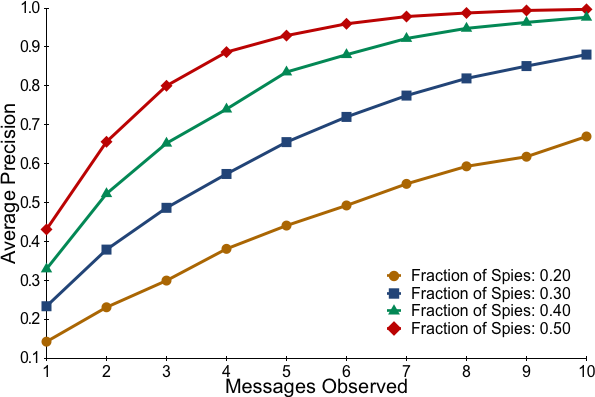
\includegraphics[width=0.7\textwidth]{images/gossip_attack.png}
    \caption{Capacità di identificazione degli IP con protocollo \textit{gossip} su rete Bitcoin}
    \source{\href{https://github.com/bitcoin/bips/blob/master/bip-0156.mediawiki}{BIP 156}}
\end{figure}
Il nuovo protocollo, \textit{Dandelion} e la sua evoluzione \textit{Dandelion++}, modificano la metodologia di comunicazione e diffusione dei messaggi dei client con gli altri. La comunicazione avviene tramite due fasi:
\begin{itemize}
    \item fase \textbf{stem}: il client invia ad un singolo nodo la transazione; i nodo destinatario procede con la stessa tecnica (\textit{1-1})
    \item fase \textbf{fluff}: dopo un tempo aleatorio la transazione viene inviata nella rete tramite \textit{broadcast}.
\end{itemize}
\begin{figure}[H]
    \centering
    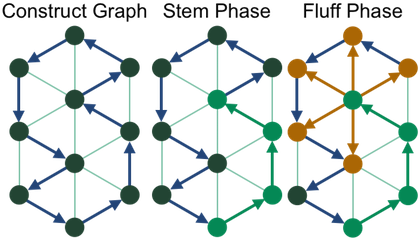
\includegraphics[width=0.6\textwidth]{images/dandelion.png}
    \caption{Fasi del protocollo \textit{Dandelion} e \textit{Dandelion++} proposto da Giulia Fanti}
    \source{\href{https://github.com/bitcoin/bips/blob/master/bip-0156.mediawiki}{BIP 156}}
\end{figure}
I \textit{peer} connessi alla rete Bitcoin possono essere di due tipi:
\begin{itemize}
    \item completi (\textit{full node})
    \item parziali (\textit{lightweight} o \textit{Simple Payment Verification})
\end{itemize}
I full node sono i nodi che si occupano di aggiornare, validare e mantenere l'intera blockchain. Nel momento in cui un full node viene connesso alla rete è necessario che scarichi, dagli altri full node, l'intera blockchain dal blocco genesi all'ultimo appena inserito e che validi tutte le transazioni inserite nonchè tener traccia delle transazioni UTXO.\newline
A Ottobre 2018 la dimensione dell'intera blockchain per Bitcoin è di $188.3$ GB. Mentre le transazioni UTXO sono circa $57$ milioni su un totale di $352$ milioni di transazioni.
\begin{figure}[H]
    \centering
    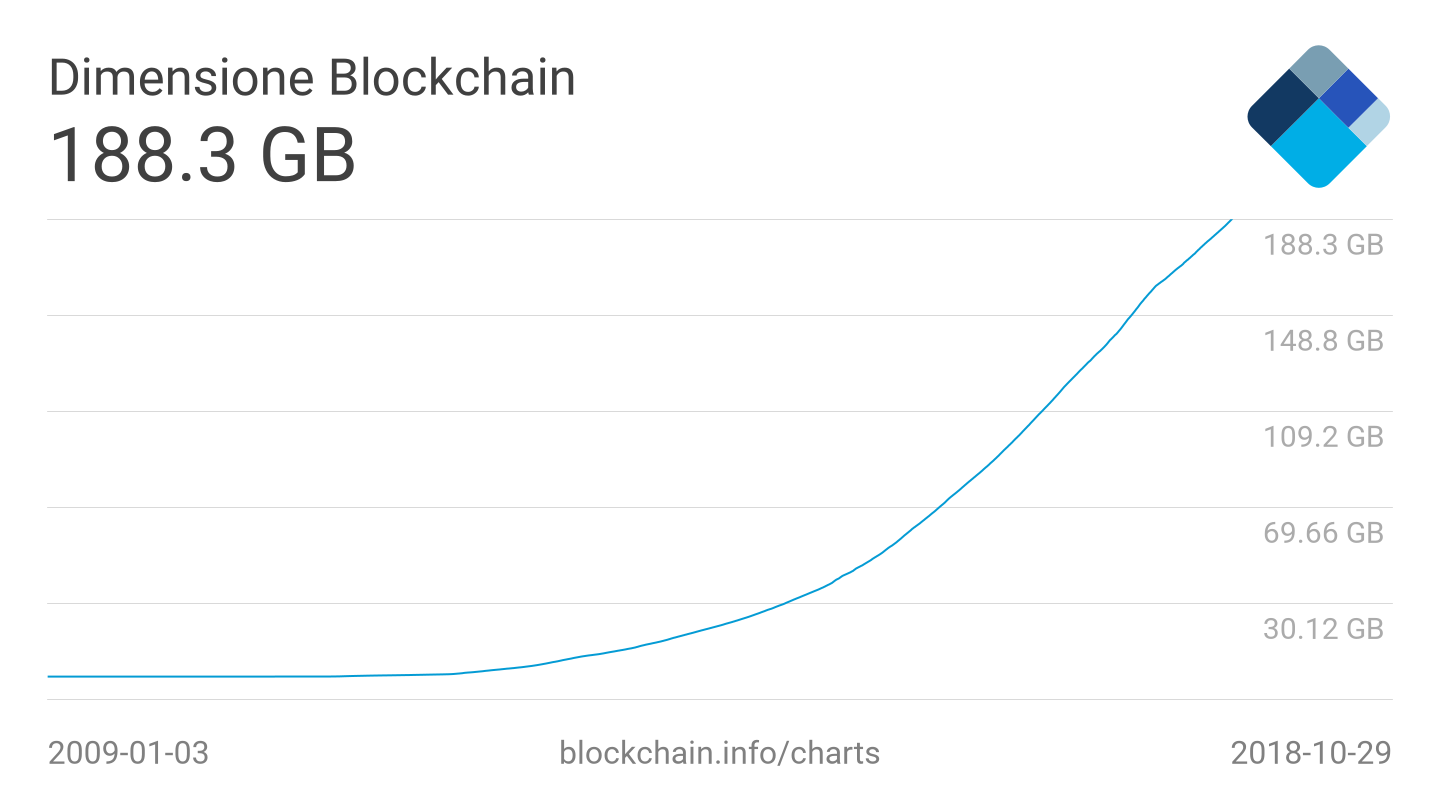
\includegraphics[width=0.75\textwidth]{images/bcsize.png}
    \caption{Grafico tempo/byte della dimensione della blockchain per Bitcoin.}
\end{figure}
Un nodo full node si occupa quindi di:
\begin{itemize}
    \item rimanere in ascolto per ricevere transazioni dai peer validandole;
    \item mantenere in locale l'intera blockchain aggiornandola con ogni nuovo blocco inserito e validato;
    \item creare un blocco candidato all'inserimento, successivo all'ultimo inserito, con le transazioni ricevute dalla rete o create in locale;
    \item trovare il \textit{nonce} per la validazione del blocco (\textbf{mining});
    \begin{itemize}
        \item se è stato trovato il nonce è necessario pubblicare sulla rete (come per le transazioni) il blocco;
        \item se il blocco trovato viene accettato dagli altri peer ed inserito nella blockchain si ha diritto ad un ricompensa;
        \item se il blocco è stato accettato gli altri peer aggiorneranno la loro blockchain;
        \item se il blocco è stato rifiutato perché non valido o perché un gli altri peer hanno già accettato un blocco alternativo allora va aggiornata la blockchain.
    \end{itemize}
\end{itemize}
I nodi \textit{lightweight} invece non hanno bisogno di conoscere l'intera blockchain ma solo le transazioni a cui sono interessati. Ad esempio la maggior parte dei software per wallet sono nodi SPV che scaricano solo i blocchi e le transazioni associate alla chiave privata del wallet.\newline
I nodi SPV non contribuiscono in maniera attiva alla sicurezza della rete Bitcoin in quanto non validano tutte le transazioni ed i blocchi ma fanno affidamento sui full node per utilizzare dei dati considerati sicuri. Questo concetto è molto importante in quanto non va ad influire sulla sicurezza della rete stessa in quanto è altamente improbabile che dei full node diffondano dei blocchi non validi con il rischio di essere rifiutati e non percepire la ricompensa per il \textbf{mining} del blocco.\newline
Un full node è l'unico modo per utilizzare la rete Bitcoin in maniera ``trustless'': validando ogni transazione e blocco è possibile controllare che tutte le regole del protocollo siano rispettate, per esempio che non ci siano transazioni di Bitcoin da utenti che non posseggono valuta. In aggiunta è anche il metodo consigliato per utilizzare Bitcoin in maniera privata ed affidabile: non è necessario pubblicare il proprio indirizzo (i client SPV devono richiedere i blocchi associati ad un wallet), non sono soggetti ad alcuni attacchi per nodi lightweight e permettono di contribuire attivamente alla rete a discapito di consumo di risorse.

\section{Mining}
Affinchè un blocco possa essere inserito nella blockchain è necessario che sia validato e che sia dimostrato di aver trovato un \textit{nonce} $x$ tale per cui $h(k||x)<T$; con $T$ il valore del target fissato (un numero a $256$ bit) e $k$ l'hash del blocco. Questo processo è chiamato \textit{prova di Bernoulli} o \textbf{mining}.\newline
Questa operazione è quella che richiede più tempo e risorse di computazione e che permette ai \textit{miner} di ricevere una ricompensa.\newline
La ricompensa è utilizzata come incentivo a mantenere attiva la rete e per creare nuovi token Bitcoin tramite una transazione coinbase. Assieme al valore della ricompensa i miner ricevono tutte le \textit{fee} delle transazioni che sono state aggiunte al blocco: una transazione con una \textti{fee} maggiore avrà molta più probabilità di essere inserita nel blocco più immediato. Ad esempio con una fee pari a $0.63\$$ la transazione è accettata e inserita nella blockchain come valida dopo circa 10 minuti, per $0.60\$$ invece il tempo medio di attesa è di circa 1 ora.\newline
Una volta trovato il nonce e pubblicato il blocco non è certo che esso venga inserito come blocco nella blockchain: il blocco deve essere valido, gli altri miner devono accettarlo aggiungendolo alla propria blockchain ed iniziare la costruzione di un nuovo blocco partendo da quest'ultimo. Se due blocchi, validi ma diversi, vengono propagati sulla rete solamente uno di essi verrà inserito nella blockchain. Quando un peer aggiunge un blocco $b$ alla propria blockchain essa sarà quella più aggiornata e di dimensione maggiore rispetto a quella degli altri peer. Nel frangente di tempo in cui il nuovo blocco $b$ è distribuito sulla rete è possibile che un altro peer aggiunga alla propria blockchain un blocco $b^{'}$, diverso da $b$. I peer che ricevono dalla rete il blocco $b^{'}$ dopo $b$ lo rifiuteranno in quanto invalido (il campo $previousHash$ non è valido); di conseguenza tutte le transazioni che non sono inserite in $b$ non faranno parte della blockchain. Il concetto alla base per cui viene rifiutato è che la blockchain valida è quella di lunghezza maggiore; in altre parole la topologia della rete e la latenza tra i peer ha un peso importante nel ricavo della ricompensa. È però necessario specificare che la possibilità che una transazione sia nel blocco $b^{'}$ e non nel blocco $b$ è molto bassa in quanto una volta propagata la transazione nella rete p2p è altamente improbabile che il nodo che ha pubblicato il blocco $b$ non abbia ricevuto il messaggio.\newline
Un full node, una volta creato il nuovo blocco con l'header che punta al nodo precedente e creato l'albero delle transazioni, tramite l'algoritmo di hashing \textbf{Hashcash} esegue queste operazioni:
\begin{enumerate}
    \item all'interno dell'header viene inserito il campo \textit{nonce} inizializzato a 0;
    \item assieme agli altri componenti (\texttt{previousHash}, \texttt{merkle\_root}, \texttt{version}, \texttt{timestamp}, \texttt{target}) viene creato un hash dell'header del blocco tramite l'algoritmo di hashing Hashcash.
    \item se l'hash prodotto è minore o uguale del target allora il blocco è valido ed è possibile pubblicarlo sulla rete;
    \item se l'hash prodotto non è valido il nonce viene incrementato di un bit e ricalcolato l'hash;
    \item se per tutti i $2^{32}$ valori del nonce non è stato trovato un hash accettabile allora è possibile cambiare il nonce all'interno della transazione coinbase e ricalcolare l'hash (in questo caso la modifica è apportata dal nuvo valore di \texttt{merkle\_root}) e si ripetono i passaggi dal punto 1.
\end{enumerate}
\begin{figure}[H]
    \centering
    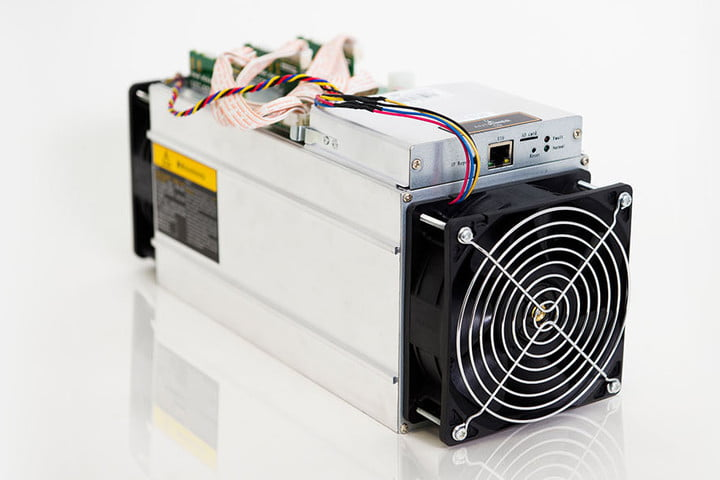
\includegraphics[width=0.7\textwidth]{images/asic.jpg}
    \caption{Un Application-Specific Integrated Circuit (ASIC) è un dispositivo progettato per effettuare efficientemente solo una operazione. ASIC per il mining dei Bitcoin hanno un hash-rate di circa $13.5$ TeraHash per secondo; un PC desktop medio raggiunge circa i 20 Megahash/s.}
    \source{BitMain}
\end{figure}
Queste operazioni sono molto onerose dal punto di vista computazionale ed per questo che molti miner e produttori sono alla ricerca di hardware sempre più specializzato ed efficiente per ottenere dei guadagni maggiori. Nonostante la potenza di calcolo abbia un ruolo molto importante non è scontato che il miner più veloce ottenga per primo un nonce valido: i blocchi su cui i miner lavorano sono sempre diversi e per le proprietà delle funzioni di hashing non è possibile prevedere quale nonce sia corretto prima di calcolarlo\footnote{Per assurdo è possibile che un miner scelga randomicamente un nonce corretto dall'inizio senza bisogno di iterazioni.}. L'operazione di verifica invece risulta immediata in quanto conoscendo il nonce è molto efficiente controllarne la correttezza.\newline
\begin{figure}
    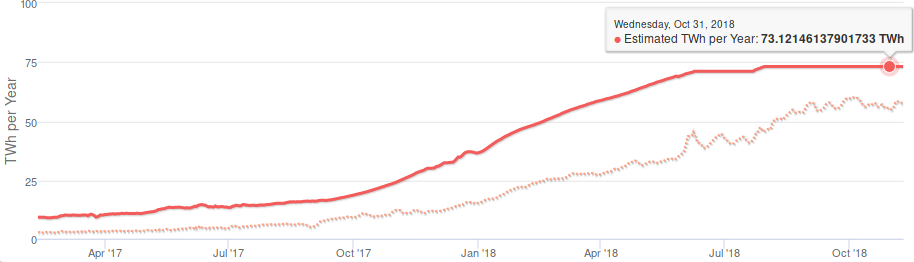
\includegraphics[width=\textwidth]{images/bitcoin_watt.png}
    \caption{Consumo stimato in \textit{TWh} dedicato al mining di Bitcoin da Febbraio 2017 a Novembre 2018.}
    \source{Digiconomist}
\end{figure}
La \textbf{difficoltà} e, di conseguenza, il target regolano la frequenza con cui i blocchi sono calcolati ed aggiunti alla blockchain in base alla totale potenza di calcolo della rete. La difficoltà viene aggiornata ogni $2016$ blocchi (circa due settimane o $20160$ minuti) al fine di avere un nuovo blocco ogni circa 10 minuti; in quanto il timestamp è leggibile per ciascun blocco ogni nodo saprà quale sarà la nuova difficoltà secondo la formula:
\begin{equation}
     difficulty = original\_target / target
\end{equation}
dove \texttt{original\_target} è il target del blocco di genesi e vale:
\begin{equation}
    00000000ffff0000000000000000000000000000000000000000000000000000
\end{equation}
Il calcolo della nuova difficoltà è effettuato da ciascun nodo e prende in considerazione il tempo $T$, totale dato dai timestamp di calcolo di 2016 blocchi, e la precedente difficoltà $D$:
\begin{equation}
    D_{next} = (20160 / T) * D
\end{equation}
Satoshi non ha specificato la durata media di calcolo di un blocco seguendo qualche regola matematica ma ha ritenuto che fosse un tempo accettabile sia dai miner che dagli utilizzatori della rete.\newline
L'attuale valore di difficoltà della rete è di $7182852313938$ volte maggiore rispetto a quella del blocco di genesi.
\begin{figure}[H]
    \centering
    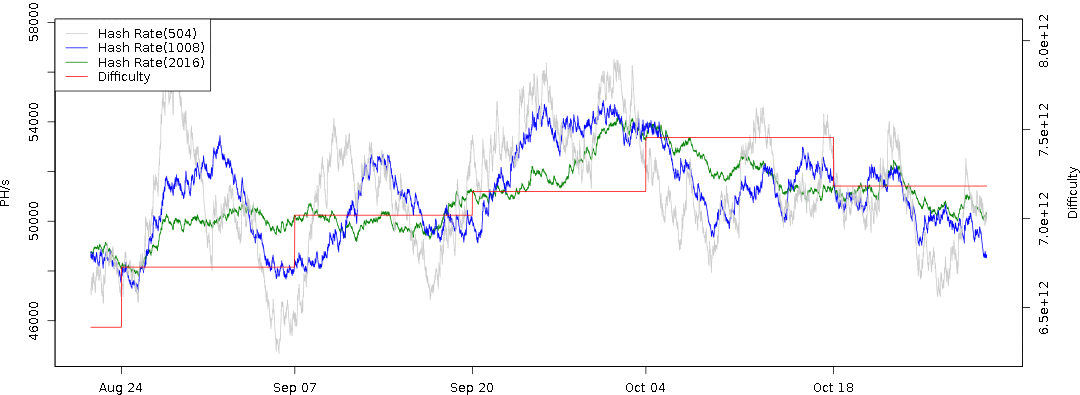
\includegraphics[width=\textwidth]{images/diffvshash.png}
    \caption{Andamento hashrate/difficoltà degli ultimi due mesi (Ottobre, 2018).}
    \source{bitcoinwisdom.com}
\end{figure}
L'incremento della difficoltà è dovuto alla crescente popolarità dei Bitcoin che porta maggiori utenti a credere nel progetto di Satoshi e quindi a farne aumentare il valore in termini di cambio BTC/\$. Un maggior valore di cambio comporta anche una maggior partecipazione dei miner che, apportando nuova potenza di calcolo alla rete, influenzano il valore della difficoltà.
\begin{figure}[H]
    \centering
    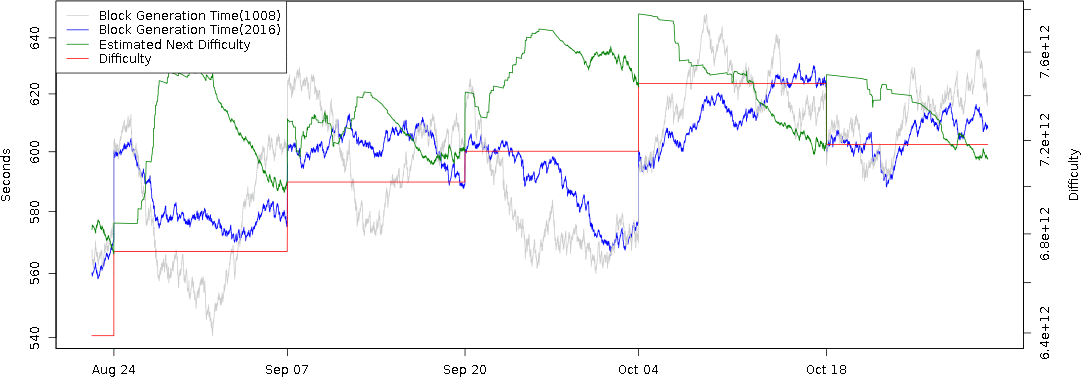
\includegraphics[width=\textwidth]{images/diffvsblock.png}
    \caption{Tempo di calcolo di un blocco (Ottobre, 2018).}
    \source{bitcoinwisdom.com}
\end{figure}
La probabilità di trovare il \textit{nonce} in un tempo $T$ (minuti) è:
\begin{equation}
    P = \exp^{-T/10}
\end{equation}
Quindi, per $10$ minuti la percentuale è del $63\%$ e per $T=7$ la percentuale di trovare il nome entro questo tempo è del $50\%$. Nelle attuali condizioni della rete la probabilità di calcolare un blocco entro i $10$ minuti ($600$ secondi) è data dalla formula:
\begin{equation}
    P_h = H * 600/(2^{32}*D)
\end{equation}
Con $H$ l'hashrate (in $H/s$) del miner e $D$ la difficoltà attuale della rete.\newline
La presenza di un limite massimo di Bitcoin in circolazione e il dimezzamento costante della \textit{reward} dato dalle attività di \texit{mining} comporta un notevole incentivo ad investire nella moneta. Satoshi non ha mai esplicitamente dichiarato il perché di un limite massimo nella produzione di Bitcoin ma è possibile giustificarlo come il valore massimo e abbastanza vicino alla rappresentazione dei numeri utilizzando una notazione a 64-bit e per evitare che la moneta venga inflazionata. In aggiunta un limite massimo comporta una speculazione maggiore tra miner ed investitori e quindi un aumento di valore più rapido.\newline
Il calcolo del limite è effettuato tenendo conto che ogni blocco viene aggiunto alla blockchain in media ogni 10 minuti e che la minima unità spendibile è di $0.00000001$ (ovvero $1$ Satoshi) con un dimezzamento ogni $210000$ blocchi. Partendo quindi dal \textit{reward} iniziale di $50$ BTC è possibile continuare a dimezzarlo fino ad arrivare ad un numero di Bitcoin che non è possibile spendere e quindi ricevere tramite una transazione coinbase.
\begin{equation}\label{eq:maxbtc}
    50 * 210000 + 50/2 * 210000 + 50/4 * 210000 + \dots + 50/n * 210000 = 210000 * \sum_{i=0}^{n} \frac{50}{2^{i}}
\end{equation}
Una volta raggiunto $n=32$ per cui il \textit{reward} per il mining non potrà più essere dimezzato (minore di un Satoshi), il totale della somma \ref{eq:maxbtc} compone il totale di Bitcoin disponibili: $20999999.9769$ (arrotondato per la rappresentazione a virgola mobile).
Il calcolo esatto diventa:
\begin{equation}
    210000 * \sum_{i=0}^{32} \frac{50}{2^{i}}  = 210000 * 99.99999997671694 = 20999999.995110556
\end{equation}
In quanto però la difficoltà è in costante aumento il limite di disponibilità dei Bitcoin risulta essere un asintoto che molti ritengono non possa essere mai raggiunto.

\subsection{Hashcash e Proof-Of-Work}
L'algoritmo \textit{Hashcash} utilizzato per generare l'hash target per ciascun blocco della blockchain Bitcoin si basa sulla proprietà crittografica delle funzioni di hashing per cui risulta essere computazionalmente inefficiente il calcolo di $x$ conoscendo $y=H(x)$. Il totale dei tentativi necessari a trovare $x$ ha come difficoltà $O(2^k)$ con $k=256$ nel caso di SHA-256 (utilizzato come algoritmo di mining per Bitcoin).\newline
Inizialmente \textit{Hashcash} fu proposto nel 1997 da \textit{Adam Black} come sistema per bloccare le email di spam o attacchi di \textit{Denial of Service} (\textit{DoS}) tramite un computazione di SHA1 per ogni messaggio o richiesta effettuata; in questo modo, per uno spammer, ad esempio, non risulta efficiente l'invio di molte mail.\newline
L'algoritmo di \textit{Hashcash} proposto da Satoshi Nakamoto prevede che gli hash già computati non possano essere riutilizzati in modo tale che i vari tentativi di mining non vengano riutilizzati; per questo viene applicato due volte SHA-256 a valori estremamente variabili. L'algoritmo prevede l'applicazione della formula: $SHA256(SHA256(s,x,c))<2^{256-k}$; con $s$ il valore inserito all'interno della transazione coinbase, $x$ l'hash dell'header del blocco, $c$ il nonce aggiornato ad ogni iterazione e $k$ il numero di bit a $0$ dell'hash target.\newline
La semplicità dell'algoritmo ha portato allo sviluppo di hardware specializzato progettato per garantire il massimo dell'efficienza dei calcoli. I miner, infatti, sono passati dall'utilizzo delle CPU general purpose ai coprocessori utilizzati nelle GPU (tramite ad esempio l'utilizzo di \textit{CUDA}) a \textit{FPGA} e \textit{ASIC} (\textit{application-specific integrated circuit}) per aumentare le possibilità di successo di costruzione di un blocco.\newline
\begin{lstlisting}[caption=Pseudocodice dell'algoritmo di mining per Hashcash]
TARGET = (65535 << 208) / DIFFICULTY
coinbase_nonce = 0
while True {
    header = makeBlockHeader(transaction, coinbase_nonce);
    for header_nonce in range(0, 2^32) {
        if (SHA256(SHA256(makeBlock(header, header_nonce))) < TARGET)
            break;
        else
            continue;
    }
    coinbase_nonce++;
}
\end{lstlisting}
Il tempo occupato dai vari miner della rete per trovare il nonce e pubblicare il nuovo blocco per avere in cambio dei Bitcoin funziona come incentivo a mantenere attiva la rete, a pubblicare blocchi che non siano stati manomessi (gli altri nodi li rifiuteranno in quanto non riusciranno a formare una blockchain più lunga di quella in possesso degli altri nodi) e a garantire che il consenso e la decentralizzazione siano efficaci e non creare situazioni di monopolio. Questa impostazione di lavoro nell'ambito delle criptomonete viene chiamato \textbf{proof-of-work} o più semplicemente \textbf{POW}. Il concetto alla base del POW consiste nel far competere i vari nodi utilizzando le proprie risorse di calcolo: per ottenere più BTC sono necessari più investimenti in hardware specializzato, il maggior numero di transazioni inserite in un blocco e quindi avere più probabilità che il blocco venga inserito nella blockchain. Di conseguenza è possibile affermare che molti attacchi su Bitcoin sono infattibili in quanto se la maggior parte dei miner, in ordine di potenza di mining, seguono le regole della rete (o sono considerati ``onesti'') si avrà una percentuale di almeno del $50\%$ che il blocco proposto provenga da un nodo ``onesto''.\newnline\newline
Considerando ad esempio un attacco chiamato \textit{double-spending} in cui un nodo, malevolo, pubblica nella rete un blocco con all'interno una transazione per un pagamento di un servizio verso Bob. Una volta ricevuta la conferma del pagamento da Bob, l'attaccante crea ed inizia a lavorare ad un nuovo blocco, dello stesso indice del precedente, ma al posto della transazione verso Bob viene inserita una transazione contrastante (ad esempio una transazione per il pagamento di un altro servizio o verso un altro wallet dell'attaccante). Così facendo l'attaccante tenta di dividere la blockchain (\textit{fork}): una branch della catena, più lunga, contiene la transazione verso Bob, l'altra branch contiene il blocco con la transazione a favore dell'attaccante. Se però tutti gli altri nodi rifiutano la seconda transazione l'attacco non ha successo.
\begin{figure}[H]
    \centering
    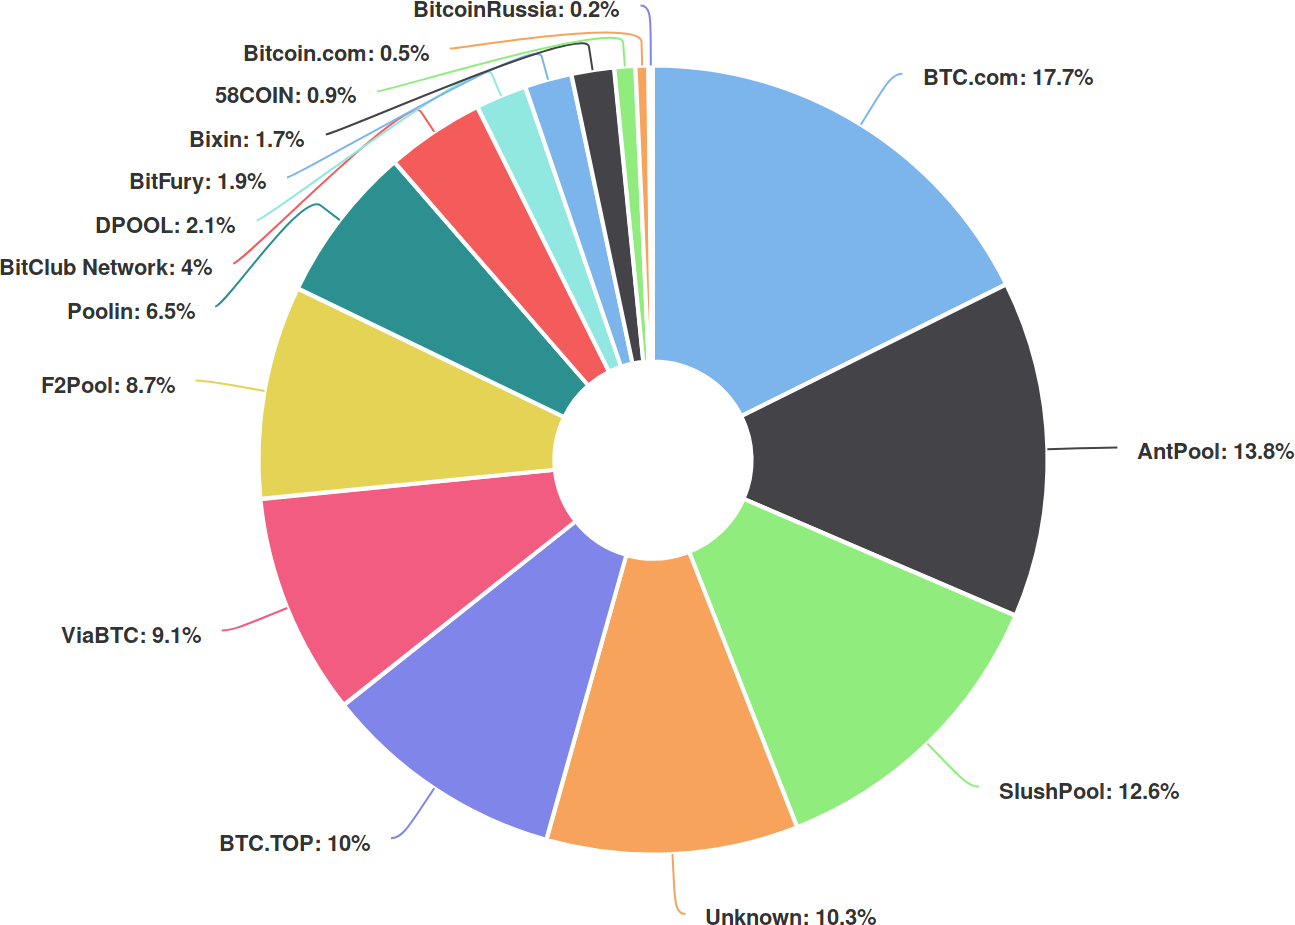
\includegraphics[width=0.8\textwidth]{images/hashratedistribution.png}
    \caption{Suddivisione della potenza di hashing tra i vari pool ad Ottobre 2018.}
    \source{acolyer.org}
\end{figure}
Le maggiori potenze di hashing rilevate sono tutte associate a dei \textit{pool} di mining: anziché tentare di trovare un nonce valido con le proprie capacità computazionali i miner si aggregano per dividere il carico di lavoro e ad aumentare le possibilità di guadagno. I \textit{pool} permettono di suddividere la ricerca del nonce tra i vari miner; in questo modo la potenza computazionale totale sarà sufficiente da risolvere il puzzle in un tempo molto minore rispetto ad un singolo miner. Una volta che all'indirizzo del \textit{pool} viene accreditata la ricompensa per il mining questa sarà suddivisa internamente tra i vari utenti in percentuale alla loro potenza di calcolo o equamente.

% NeoTex: mainfile=main.tex:
